
% =====================================================================
\chapter{Phân tích yêu cầu và thiết kế khung giải pháp}
\label{ch:thiet-ke}
\label{ch:design} % Bí danh để các chương khác tham chiếu theo tên tiếng Anh

Chương 3 đã thiết lập nền tảng lý thuyết về kiến trúc Transformer, các mô hình PhoBERT và mGTE, mạng Siamese, các thuật toán hình học không gian trong PostGIS và mô hình Điểm tin cậy địa chỉ. Chương này vận dụng các nền tảng đó để cụ thể hóa khung giải pháp \textbf{VN Address Intelligence} (VNAI) trên hai phương diện: phân tích yêu cầu hệ thống và thiết kế chi tiết bốn module chức năng. Trọng tâm của chương là pipeline AI toàn diện, bao gồm thu nạp dữ liệu đa nguồn, huấn luyện mô hình NER, kiến trúc retrieval đa tầng và logic suy luận của tầng LLM trong việc xử lý các biến động hành chính phức tạp.

% ---------------------------------------------------------------------
\section{Phân tích yêu cầu hệ thống}
\label{sec:yeu-cau}

\subsection{Yêu cầu nghiệp vụ}
\label{sec:business-req}

Khung giải pháp VNAI được đặt trong bối cảnh chuyển đổi hành chính 2025 với mục tiêu phục vụ đồng thời các nhóm tác vụ nghiệp vụ logistics, thương mại điện tử và quản lý hành chính công. Phân tích các kịch bản vận hành thực tế cho phép xác định sáu yêu cầu nghiệp vụ (Business Requirements --- BR) cốt lõi.

\begin{itemize}[leftmargin=*]
\item \textbf{BR1 --- Đồng bộ hành chính.} Hệ thống phải chủ động cập nhật danh mục đơn vị hành chính từ nguồn Chính phủ (NSO --- General Statistics Office) mà không cần can thiệp thủ công, đảm bảo dữ liệu hành chính trong kho luôn đồng bộ với văn bản pháp lý hiện hành.
\item \textbf{BR2 --- Chuẩn hóa địa chỉ thô.} Hệ thống tiếp nhận đầu vào là chuỗi địa chỉ tự do (freetext), trả về cấu trúc chuẩn hóa kèm mã định danh đơn vị hành chính ba cấp.
\item \textbf{BR3 --- Quản lý lịch sử hành chính.} Hệ thống cho phép tra cứu trạng thái của một đơn vị hành chính tại bất kỳ thời điểm nào trong lịch sử, hỗ trợ ánh xạ địa chỉ tiền cải cách sang định danh hậu cải cách.
\item \textbf{BR4 --- Xác định không gian.} Với đầu vào là tọa độ (latitude, longitude), hệ thống xác định chính xác đơn vị hành chính chứa điểm đó, đặc biệt tại các vùng ranh giới tiếp giáp.
\item \textbf{BR5 --- Làm giàu dữ liệu.} Hệ thống tự động bổ sung tọa độ, ranh giới đa giác, tên điểm quan tâm (Point of Interest --- POI) từ các nguồn mở (OpenStreetMap, Google Maps) vào hồ sơ địa chỉ.
\item \textbf{BR6 --- Benchmark liên tục.} Hệ thống cung cấp nền tảng so sánh hiệu năng giữa các mô hình AI theo thời gian, hỗ trợ ra quyết định lựa chọn mô hình triển khai.
\end{itemize}

\subsection{Yêu cầu phi chức năng}
\label{sec:non-functional}

Bốn nhóm yêu cầu phi chức năng (Non-Functional Requirements --- NFR) định hình các ràng buộc kỹ thuật của khung giải pháp. Thứ nhất, về hiệu năng, độ trễ trung bình cho một yêu cầu chuẩn hóa đơn lẻ phải dưới 200ms, độ trễ ở phân vị 95 (P95) dưới 500ms, và lưu lượng xử lý đạt ít nhất 20 địa chỉ trên giây ở chế độ batch. Thứ hai, về khả năng mở rộng, kiến trúc phải tuân theo mô hình microservices cho phép mở rộng theo chiều ngang (horizontal scaling) khi tải tăng. Thứ ba, về tính chính xác, mục tiêu chỉ số F1 trên tập kiểm thử 10.000 mẫu đa dạng đạt ít nhất 85\%. Thứ tư, về tính sẵn sàng, hệ thống đồng bộ hành chính hoạt động theo lịch định kỳ (cron) hoặc trigger sự kiện khi có thay đổi từ nguồn pháp lý.

Ngoài bốn nhóm trên, khung giải pháp ưu tiên ba ràng buộc kỹ thuật chiến lược: triển khai \thuat{self-hosted} với toàn bộ thành phần mã nguồn mở để loại trừ phụ thuộc vào dịch vụ thương mại bên thứ ba; đảm bảo khả năng truy vết nguồn gốc (provenance) cho mọi bản ghi địa chỉ thông qua các cột audit; và duy trì cơ chế tái lập (reproducibility) cho mọi thực nghiệm khoa học.

\subsection{Phân tích luồng dữ liệu}
\label{sec:data-flow}

Hệ thống vận hành theo năm luồng dữ liệu chính, tổng hợp tại \cref{tab:data-flows}. Năm luồng này liên kết với nhau qua kho dữ liệu trung tâm PostgreSQL nhưng được thiết kế độc lập về mặt khởi tạo và lịch chạy, cho phép vận hành mỗi luồng riêng biệt mà không ảnh hưởng các luồng còn lại.

\begin{table}[H]
\centering
\caption{Năm luồng dữ liệu chính của khung giải pháp VNAI}
\label{tab:data-flows}
\small
\begin{tabularx}{\linewidth}{>{\raggedright\arraybackslash}p{1.4cm} >{\raggedright\arraybackslash}p{4cm} >{\raggedright\arraybackslash}X}
\toprule
\textbf{Luồng} & \textbf{Tên} & \textbf{Mô tả} \\
\midrule
F1 & Đồng bộ hành chính & Government API $\to$ ETL $\to$ PostgreSQL schema \schema{mat} \\
F2 & Chuẩn hóa địa chỉ  & Raw Address $\to$ Queue \schema{prq} $\to$ AI Pipeline $\to$ Structured Output \\
F3 & Xác định không gian & Coordinates $\to$ PostGIS \macode{ST\_Contains} $\to$ Admin Unit \\
F4 & Làm giàu dữ liệu   & Standardized Address $\to$ OSM/Google $\to$ Enriched Address \\
F5 & Benchmarking       & Test Set $\to$ AI Models $\to$ Metrics $\to$ schema \schema{ath} \\
\bottomrule
\end{tabularx}
\end{table}

% ---------------------------------------------------------------------
\section{Kiến trúc tổng thể VNAI}
\label{sec:kien-truc}

\subsection{Triết lý thiết kế}
\label{sec:triet-ly}

Bốn nguyên tắc thiết kế cốt lõi định hướng toàn bộ kiến trúc VNAI. \emph{Tách biệt mối quan tâm (Separation of Concerns)} --- bốn module nghiệp vụ (thu thập dữ liệu, chuẩn hóa AI, xác thực không gian, làm giàu dữ liệu) được hiện thực thành các thành phần độc lập, giao tiếp qua hợp đồng dữ liệu (data contract) rõ ràng thông qua các schema PostgreSQL chuyên biệt. \emph{Kho tri thức làm trung tâm (Knowledge Base First)} --- cơ sở dữ liệu hành chính chuẩn trong schema \schema{mat} được xem là Nguồn sự thật duy nhất (Single Source of Truth); mọi mô hình AI tra cứu Knowledge Base thay vì sinh (\thuat{hallucinate}) địa danh, qua đó loại trừ rủi ro tạo ra các định danh không tồn tại.

\emph{Nhận thức thời gian (Temporal Awareness)} --- mọi thực thể hành chính đều mang thông tin thời gian theo mô hình Slowly Changing Dimension (SCD) Type 2, cho phép truy vết các phiên bản hành chính cũ và mới song song. \emph{Truy xuất lai (Hybrid Retrieval)} --- hệ thống kết hợp tìm kiếm từ vựng (Typesense BM25) với tìm kiếm ngữ nghĩa (mGTE/Siamese embedding) và Late Interaction để cân bằng giữa tốc độ và độ chính xác.

\subsection{Công nghệ (Technology Stack)}
\label{sec:tech-stack}

Khung giải pháp được hiện thực trên Python 3.11+, với các thành phần phần mềm được tổ chức thành sáu lớp như tóm lược tại \cref{tab:tech-stack}. Việc lựa chọn các thành phần này dựa trên ba tiêu chí: mã nguồn mở để phù hợp chiến lược tự chủ hạ tầng; hỗ trợ tốt cho tiếng Việt; và khả năng tích hợp với hệ sinh thái học sâu PyTorch + Hugging Face.

\begin{table}[H]
\centering
\caption{Chồng công nghệ phân lớp của khung giải pháp VNAI}
\label{tab:tech-stack}
\small
\begin{tabularx}{\linewidth}{>{\raggedright\arraybackslash}p{3.2cm} >{\raggedright\arraybackslash}X}
\toprule
\textbf{Lớp} & \textbf{Thành phần} \\
\midrule
Lõi và truy cập dữ liệu & SQLAlchemy 2+, psycopg2-binary, python-dotenv, click, tqdm, PyYAML, psutil \\
Dịch vụ web & FastAPI \cite{Tiangolo2024FastAPI}, Uvicorn, Gunicorn, httpx, PyJWT, passlib (bcrypt) \\
Học máy và NLP & PyTorch 2.4.1+, Hugging Face Transformers \cite{Wolf2020Transformers}, sentence-transformers, seqeval, scikit-learn 1.3.2, bitsandbytes, accelerate \\
Tiếng Việt & pyvi, vnaddress, VnCoreNLP (qua PhoBERT pipeline) \\
Địa lý & overpy (Overpass), Folium \cite{Folium2024}, Shapely \cite{Shapely2024}, pyproj, alphashape, PostGIS \cite{PostGIS2024} \\
Hạ tầng vận hành & Redis (cache), python-logstash-async (ELK), Docker Compose \\
\bottomrule
\end{tabularx}
\end{table}

\subsection{Kiến trúc phân lớp và cấu trúc mã nguồn}
\label{sec:layered-arch}

Khung giải pháp tuân theo kiến trúc phân lớp gồm bốn lớp: Lớp Trình bày (Presentation), Lớp Nghiệp vụ (Business / Service), Lớp AI (AI Hub) và Lớp Dữ liệu (Data). \cref{fig:layered-arch} thể hiện trực quan kiến trúc này. Tầng API chỉ điều phối: nhận yêu cầu HTTP, gọi dịch vụ nghiệp vụ hoặc module suy luận, trả về DTO (Data Transfer Object) hoặc JSON. Logic nghiệp vụ tái sử dụng dài hạn nằm trong dịch vụ domain hoặc gói AI. Script vận hành, migration và thực nghiệm được tổ chức riêng và gọi qua trình thông dịch Python thay vì \thuat{import} như thư viện nội bộ của server, qua đó loại bỏ phụ thuộc giữa kịch bản nghiên cứu và server production.
\begin{figure}[H] % Sử dụng [H] từ gói float để cố định vị trí
  \centering
  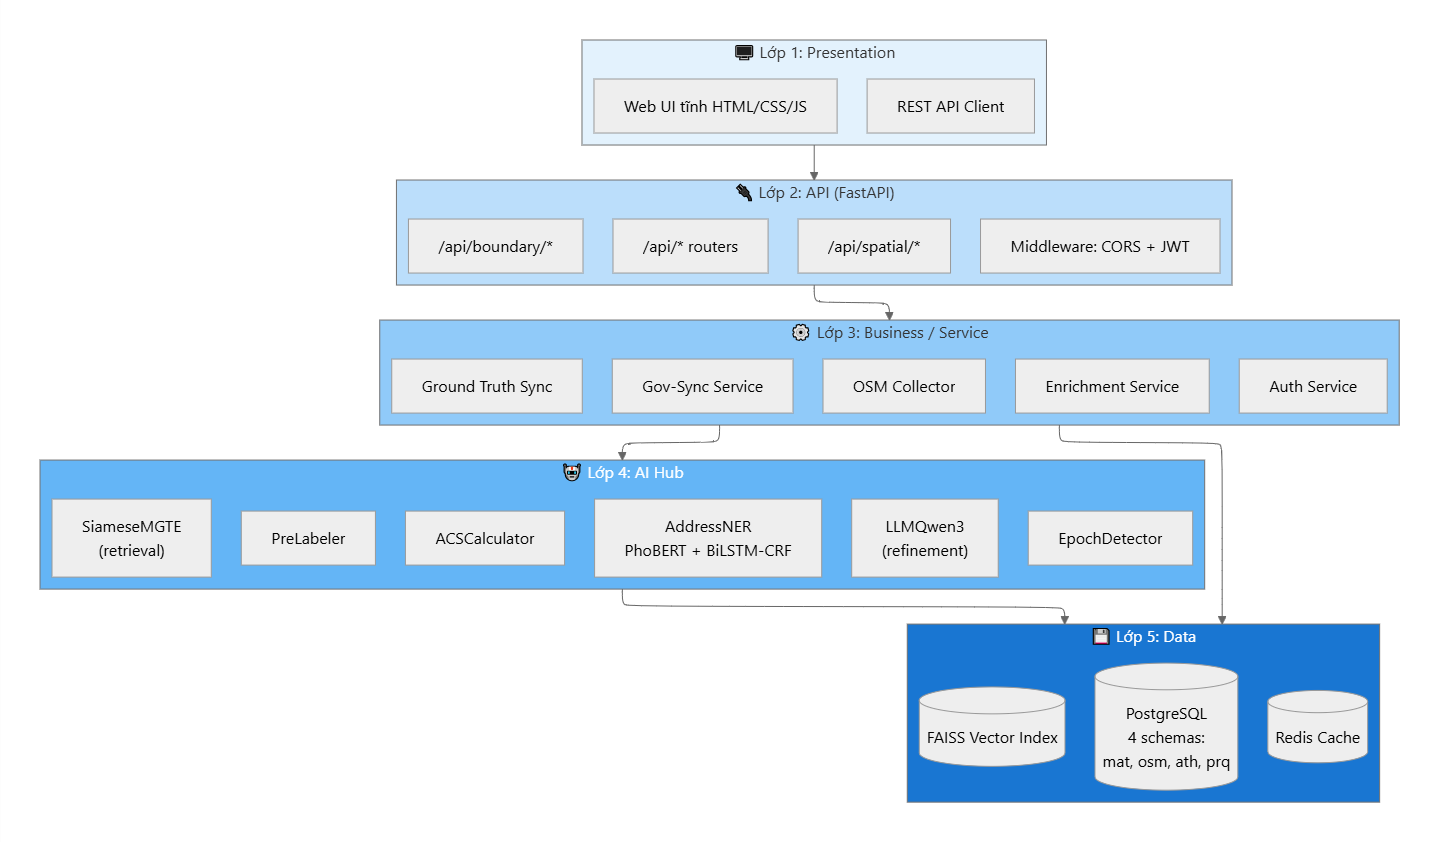
\includegraphics[width=0.8\linewidth]{figs/fig-4-1.png}
  \caption{Kiến trúc phân lớp bốn tầng của khung giải pháp VNAI.}
  \label{fig:layered-arch}
  
  \vspace{1em} % Khoảng cách nhỏ giữa 2 hình
  
  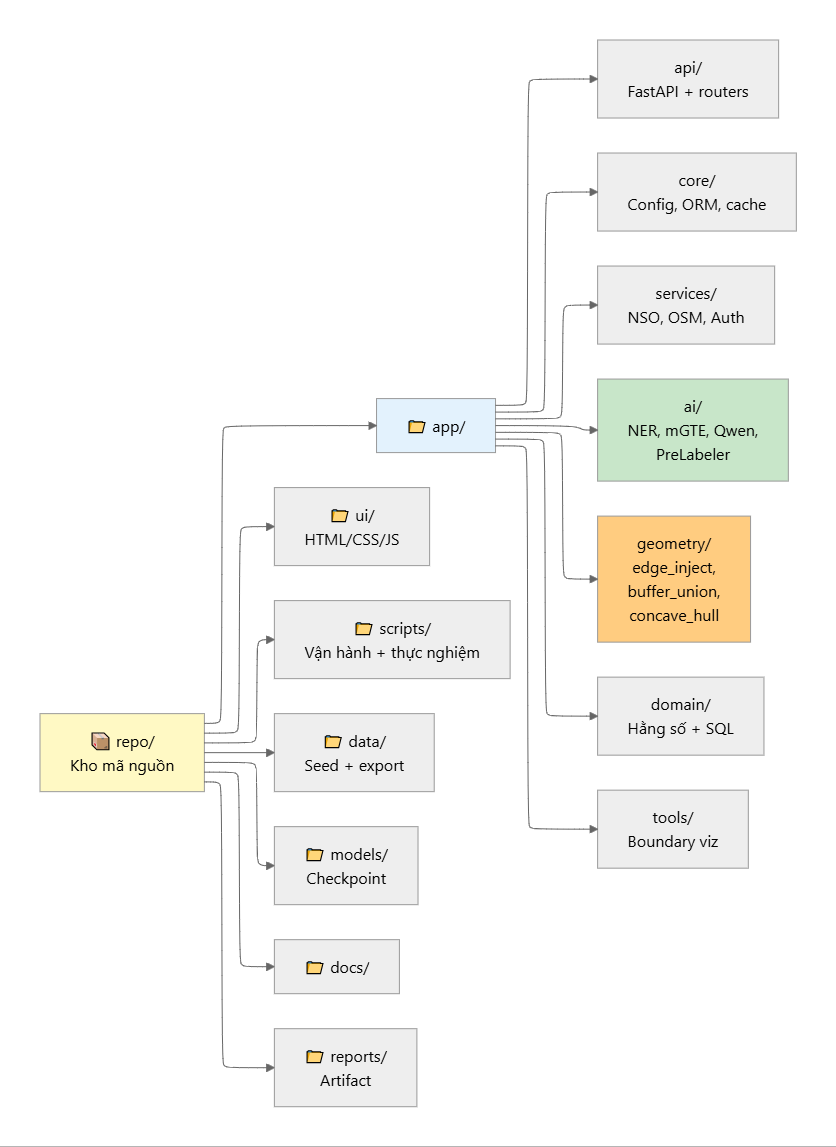
\includegraphics[width=0.4\linewidth]{figs/fig-4-2.png}
  \caption{Cấu trúc thư mục logic kho mã nguồn VNAI.}
  \label{fig:repo-structure}
\end{figure}
Bốn khối chức năng chính lần lượt là: gói \macode{api} đăng ký tập route REST, gắn middleware CORS khi cần và nạp mô hình AI trong luồng nền (background thread) để giảm độ trễ khởi động; gói \macode{services} chứa các dịch vụ đồng bộ NSO với logic SCD Type 2, thu thập OSM, làm giàu dữ liệu, xác thực người dùng và đồng bộ ground truth từ Typesense; gói \macode{ai} chứa các lớp mô hình \macode{AddressNER}, \macode{SiameseMGTE}, \macode{LLMQwen3}, script huấn luyện, pipeline production kết hợp retrieval--NER--LLM--ACS, cùng EpochDetector và PreLabeler; gói \macode{geometry} hiện thực ba chiến lược hiệu chỉnh polygon (Mục~\ref{sec:edge-inject}).

% ---------------------------------------------------------------------
\section{Thiết kế cơ sở dữ liệu đa schema}
\label{sec:csdl}

\subsection{Quy ước chung và mô hình SCD Type 2}
\label{sec:quy-uoc}

Cơ sở dữ liệu được phân tách thành bốn schema logic chuyên biệt: \schema{mat} (Master Administrative Table) cho dữ liệu đơn vị hành chính và polygon ranh giới; \schema{osm} cho thực thể OpenStreetMap đã xử lý; \schema{ath} (Analytics \& Training Hub) cho huấn luyện, benchmark, nhật ký đồng bộ; và \schema{prq} (Processing Queue) cho hàng đợi xử lý địa chỉ và ground truth. Việc tách schema giúp phân quyền vận hành theo miền dữ liệu, sao lưu chọn lọc và giảm rủi ro thay đổi lẫn nhau giữa dữ liệu nghiệp vụ và artifact thực nghiệm. \cref{fig:erd-schema} trình bày lược đồ ER (Entity-Relationship) đầy đủ cho bốn schema.

\begin{figure}[H]
\centering
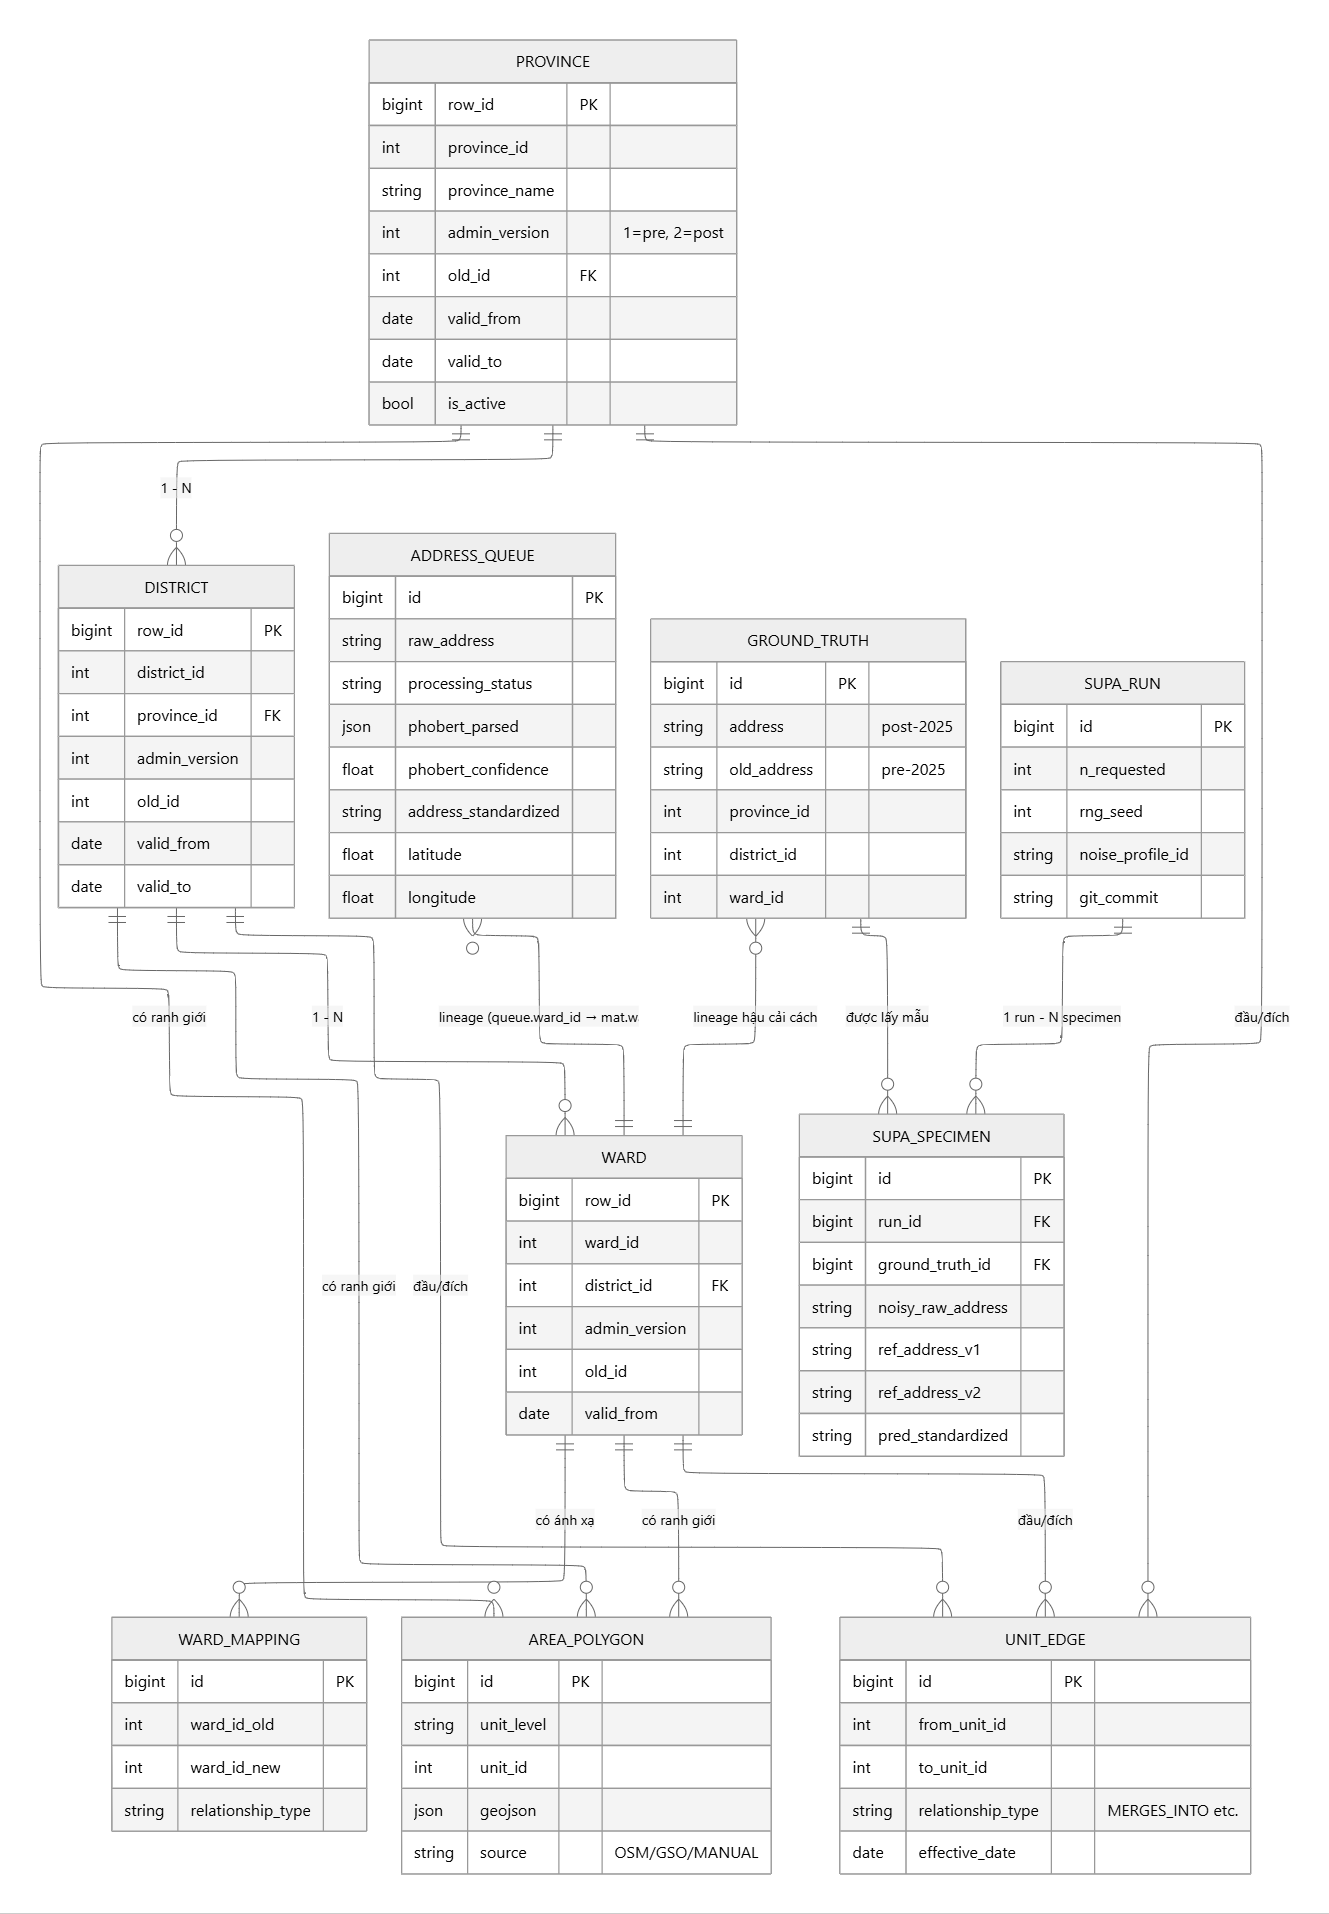
\includegraphics[width=0.5\linewidth]{figs/fig-4-3.png}
% 
% \fbox{\begin{minipage}{0.92\linewidth}\centering\vspace{1.4cm}\textit{[Hình 4.x: Lược đồ ER đầy đủ của bốn schema \texttt{mat}, \texttt{osm}, \texttt{ath}, \texttt{prq}. \textbf{Schema mat}: các bảng \texttt{province}, \texttt{district}, \texttt{ward} với khoá nghiệp vụ + cột SCD (\texttt{valid\_from/to}, \texttt{is\_active}); bảng \texttt{ward\_mapping}, \texttt{unit\_edge} thể hiện đồ thị quan hệ; \texttt{area\_polygon} lưu GeoJSON. \textbf{Schema osm}: \texttt{streets}, \texttt{buildings}, \texttt{pois}, \texttt{raw\_entities}. \textbf{Schema ath}: \texttt{training\_datasets}, \texttt{training\_history}, \texttt{benchmark\_model\_baselines}, \texttt{benchmark\_dataset}, \texttt{benchmark\_run\_result}, \texttt{sync\_log}, \texttt{supa\_stratified\_eval\_summary}. \textbf{Schema prq}: \texttt{address\_cleansing\_queue}, \texttt{ground\_truth}, \texttt{supa\_benchmark\_run}, \texttt{supa\_benchmark\_specimen}. Các cạnh PK--FK thể hiện ràng buộc tham chiếu; các cạnh đứt thể hiện liên kết lineage ngầm qua \texttt{old\_id}/\texttt{admin\_version}.]}\vspace{1.4cm}\end{minipage}}
\caption{Lược đồ ER đầy đủ của bốn schema cơ sở dữ liệu VNAI.}
\label{fig:erd-schema}
\end{figure}

Mọi bảng master tuân thủ tập quy ước cột thống nhất nhằm hiện thực mô hình SCD Type 2 \cite{kimball2013}. Cụ thể, mỗi bảng có một khóa tự sinh (\macode{row\_id}) đóng vai trò khóa chính vật lý, một mã định danh nghiệp vụ (\macode{province\_id}, \macode{district\_id}, \macode{ward\_id}) mang ý nghĩa trong miền nghiệp vụ, cột \macode{admin\_version} phân biệt phiên bản hành chính (1: tiền cải cách, 2: hậu cải cách 01/07/2025), cột \macode{old\_id} lưu định danh legacy để join ngược hệ thống cũ, cặp \macode{valid\_from}/\macode{valid\_to} cùng \macode{predecessor\_id} và \macode{version\_id} hỗ trợ truy vết lịch sử, cờ \macode{is\_active} chỉ bản ghi đại diện hiện tại cho API, và \macode{is\_deleted} đánh dấu xóa mềm.

\subsection{Schema mat --- Đơn vị hành chính và ranh giới}
\label{sec:schema-mat}

Schema \schema{mat} chứa sáu bảng cốt lõi tổ chức theo phân cấp ba tầng tỉnh--huyện--xã. \cref{tab:mat-tables} tóm lược chức năng các bảng. Trong đó, bảng \macode{mat.area\_polygon} đóng vai trò đặc biệt: lưu ranh giới đơn vị hành chính dưới dạng GeoJSON, có chỉ mục trên cặp (\macode{unit\_level}, \macode{unit\_id}), là đầu vào cho mọi truy vấn PostGIS như \macode{ST\_Contains}, \macode{ST\_Distance}.

\begin{table}[H]
\centering
\caption{Các bảng cốt lõi trong schema \schema{mat}}
\label{tab:mat-tables}
\small
\begin{tabularx}{\linewidth}{>{\raggedright\arraybackslash}p{3.6cm} >{\raggedright\arraybackslash}X}
\toprule
\textbf{Bảng} & \textbf{Vai trò} \\
\midrule
\macode{mat.province}     & Quản lý đơn vị cấp tỉnh kèm SCD, các cột bao hộp tọa độ cực, khối GSO mở rộng (population, area\_km2, decision\_number, decision\_date) \\
\macode{mat.district}     & Quản lý đơn vị cấp huyện kèm SCD; sau cải cách 2025 các bản ghi cấp huyện được đánh \macode{valid\_to} nhưng vẫn lưu cho truy vấn lịch sử \\
\macode{mat.ward}         & Quản lý đơn vị cấp xã/phường kèm SCD và mã GSO mở rộng \\
\macode{mat.ward\_mapping} & Ánh xạ chuyển đổi cấp xã: cặp \macode{ward\_id\_old/new}, khoảng hiệu lực, \macode{relationship\_type} \\
\macode{mat.unit\_edge}    & Đồ thị có hướng quan hệ đơn vị: \macode{from\_unit\_id}, \macode{to\_unit\_id}, \macode{relationship\_type} $\in$ \{MERGES\_INTO, SPLIT\_FROM, RENAMES\_TO, BOUNDARY\_ADJUSTED\} \\
\macode{mat.area\_polygon} & Ranh giới geojson cho cả ba cấp, kèm nguồn (\macode{source} $\in$ \{OSM, GSO, MANUAL\}) và \macode{admin\_version} \\
\bottomrule
\end{tabularx}
\end{table}

Đặc biệt, bảng \macode{mat.unit\_edge} hiện thực hóa khái niệm \emph{đồ thị biến động đơn vị hành chính}: khi một xã sáp nhập vào xã khác, hệ thống tạo cạnh \macode{MERGES\_INTO}; khi một huyện được tách, các cạnh \macode{SPLIT\_FROM} được tạo từ huyện gốc sang các đơn vị mới. Cấu trúc đồ thị này không chỉ phục vụ truy vết lịch sử mà còn được sử dụng trực tiếp trong thuật toán Edge Injection ở Mục~\ref{sec:edge-inject}.

\subsection{Schema osm --- Dữ liệu OpenStreetMap}
\label{sec:schema-osm}

Schema \schema{osm} chứa bốn bảng: \macode{streets}, \macode{buildings}, \macode{pois} với cấu trúc tương tự (\macode{id}, \macode{name}, \macode{type}, \macode{province\_id}, \macode{province\_name}, \macode{created\_at}), và bảng \macode{raw\_entities} lưu nguyên trạng dữ liệu OSM dưới dạng JSON với cột \macode{osm\_type} $\in$ \{node, way, relation\} và \macode{tags} JSON chứa toàn bộ cặp khóa--giá trị OSM gốc. Cách lưu trữ này cho phép hệ thống vừa truy vấn nhanh trên các bảng đã chuẩn hóa, vừa giữ nguyên dữ liệu thô để truy hồi khi cần làm giàu lại theo các trường mới.

\subsection{Schema ath --- Hub AI, benchmark và nhật ký}
\label{sec:schema-ath}

Schema \schema{ath} là trung tâm của các hoạt động học máy và đảm bảo tái lập thực nghiệm. \cref{tab:ath-tables} liệt kê các bảng chính. Đáng chú ý, cặp \macode{benchmark\_dataset} (chứa các tập kiểm thử D1--D5 theo phân loại nhiễu) và \macode{benchmark\_run\_result} (lưu mọi dự đoán của từng mô hình trên từng mẫu, kèm UUID nhóm run) hình thành nền tảng cho khung đánh giá khoa học chuẩn (Chương~\ref{ch:experiments}).

\begin{table}[H]
\centering
\caption{Các bảng cốt lõi trong schema \schema{ath}}
\label{tab:ath-tables}
\small
\begin{tabularx}{\linewidth}{>{\raggedright\arraybackslash}p{4.4cm} >{\raggedright\arraybackslash}X}
\toprule
\textbf{Bảng} & \textbf{Vai trò} \\
\midrule
\macode{training\_datasets}        & Tập huấn luyện NER với \macode{ner\_tags\_json} (BIO), cờ \macode{is\_synthetic}, mức nhiễu \\
\macode{training\_history}         & Lịch sử huấn luyện: phiên bản, F1, loss, số mẫu \\
\macode{benchmark\_model\_baselines} & Mô hình baseline với F1, throughput, chi phí/1M mẫu, \macode{google\_match} \\
\macode{benchmark\_dataset}        & Mẫu kiểm thử (D1--D5) kèm \macode{noise\_type}, \macode{admin\_version}, expected IDs \\
\macode{benchmark\_run\_result}    & Kết quả dự đoán: \macode{run\_id} (UUID), dự đoán ID, ACS, decision, epoch, latency \\
\macode{sync\_log}                  & Nhật ký đồng bộ với \macode{sync\_source} $\in$ \{NSO\_API, N8N\_WORKFLOW, MANUAL\} \\
\macode{typesense\_ground\_truth\_sync\_run} & Run đồng bộ ground truth từ Typesense \\
\macode{email\_verifications}      & Mã xác thực email cho luồng đăng ký \\
\macode{retrieval\_eval\_run}      & Lịch sử các lần chạy \macode{evaluate\_retriever} với \thuat{persist-db}: \macode{model\_name}, \macode{limit\_pairs}, \macode{top\_k\_max}, \macode{metrics\_json} (R@k, MRR, NDCG, provenance) \\
\macode{supa\_stratified\_eval\_summary} & Bảng tổng hợp các batch \texttt{replicate-stratified} K~=~5: phạm vi \macode{run\_id}, payload JSON đầy đủ, \macode{methodology\_version}, \macode{git\_commit} \\
\bottomrule
\end{tabularx}
\end{table}

\subsection{Schema prq --- Hàng đợi xử lý và ground truth}
\label{sec:schema-prq}

Schema \schema{prq} đóng vai trò hai mặt: vừa là hàng đợi xử lý cho pipeline AI sản xuất, vừa là kho ground truth phục vụ huấn luyện và đánh giá. Bảng \macode{prq.address\_cleansing\_queue} là trung tâm: chứa địa chỉ thô (\macode{raw\_address}), trạng thái xử lý (PENDING, PROCESSING, DONE, FAILED), kết quả phân tích từ cả PhoBERT (\macode{phobert\_parsed\_components} JSON, \macode{phobert\_confidence\_score}) và mGTE (\macode{mgte\_parsed\_components}, \macode{mgte\_confidence\_score}), cờ chọn mô hình\\ (\macode{selected\_ai\_model}), chuỗi chuẩn hóa cuối cùng (\macode{address\_standardized}), tọa độ làm giàu (lat/lng), và các trường lineage tiền cải cách (\macode{old\_province\_id}, \macode{old\_district\_id}, \macode{old\_ward\_id}).

Bảng \macode{prq.ground\_truth} lưu cặp địa chỉ chuẩn lưỡng thời: \macode{address} (định danh hậu cải cách, bắt buộc) và \macode{old\_address} (định danh tiền cải cách), kèm cặp ba cấp tỉnh--huyện--xã cho cả hai phiên bản. Mỗi bản ghi có cờ \macode{is\_validated}, \macode{data\_quality\_score}, và liên kết tới run đồng bộ Typesense thông qua \macode{last\_sync\_run\_id}. Đây là kho dữ liệu nền tảng cho khung thực nghiệm SUPA-Bench (Mục~\ref{sec:supa}).

\subsection{Bảng SUPA-Bench cho thực nghiệm}
\label{sec:supa-tables}

Hai bảng \macode{prq.supa\_benchmark\_run} (metadata mỗi lần chạy benchmark) và \\ \macode{prq.supa\_benchmark\_specimen} (mẫu benchmark cụ thể) được định nghĩa qua migration SQL riêng, không map đầy đủ trong ORM chính nhằm giảm cặp ràng buộc giữa ứng dụng và bảng thực nghiệm. Các trường quan trọng gồm \macode{rng\_seed} (hạt giống ngẫu nhiên), \macode{noise\_profile\_id} (mã profile nhiễu), \macode{git\_commit} (commit hash tại thời điểm extract), \macode{ref\_address\_v2}\\/\macode{ref\_address\_v1} (snapshot tham chiếu hậu/tiền cải cách), \macode{noisy\_raw\_address} (chuỗi đã nhiễu),  \macode{pred\_standardized} (dự đoán của mô hình ngoài).

\textbf{Bất biến thực nghiệm (Experimental Invariant):} pipeline SUPA-Bench tuyệt đối không thực hiện thao tác \macode{INSERT} / \macode{UPDATE} / \macode{DELETE} trên \macode{prq.ground\_truth}; mọi truy vấn chỉ là \macode{SELECT}. Bất biến này đảm bảo tính độc lập giữa pipeline thực nghiệm và kho dữ liệu tham chiếu.

% ---------------------------------------------------------------------
\section{Module 1: Đồng bộ danh mục hành chính (Gov-Sync)}
\label{sec:gov-sync}

\subsection{Luồng đồng bộ từ nguồn NSO}
\label{sec:nso-sync}

Module Gov-Sync hiện thực luồng đồng bộ tự động từ API danh mục hành chính của Tổng cục Thống kê (NSO). Client Python gọi tuần tự ba endpoint: danh sách tỉnh, danh sách huyện theo tỉnh, danh sách xã theo huyện; mỗi phản hồi được chuẩn hóa thông qua các hàm làm sạch tên (loại bỏ ký tự đặc biệt, chuẩn hóa Unicode NFC) và dịch loại đơn vị sang tiếng Anh khi cần (\macode{type\_name\_en}). Sau khi nhận được dữ liệu mới, hàm \macode{upsert\_scd} so checksum trên tập trường nghiệp vụ; khi phát hiện thay đổi có ý nghĩa, bản ghi active hiện tại được đóng (\macode{valid\_to = NOW()}, \macode{is\_active = FALSE}) và bản ghi mới được chèn với mã đơn vị nghiệp vụ bắt buộc trong payload.

REST API expose bốn endpoint cốt lõi cho module này: 
\begin{itemize}
    \item \macode{POST /api/sync/nso} kích hoạt đồng bộ toàn bộ; 
    \item \macode{POST /api/sync/nso/province} đồng bộ theo một mã tỉnh; 
    \item \macode{GET /api/sync/nso/logs} đọc log đồng bộ; 
    \item \macode{DELETE /api/sync/nso/logs} xóa log. 
     
    \item Bộ ba endpoint \macode{GET /api/nso/provinces}, \macode{/districts}, \macode{/wards} cung cấp chế độ chỉ đọc dữ liệu trực tiếp từ NSO mà không ghi DB, phục vụ kiểm tra trước khi đồng bộ chính thức.
\end{itemize}


\subsection{SCD Type 2 và đồ thị quan hệ unit\_edge}
\label{sec:scd-graph}

Mỗi thay đổi hành chính được ghi vào \macode{ath.sync\_log} với \macode{run\_id} nhóm, cho phép truy vết toàn bộ lịch sử biến động theo từng lần chạy. Đồng thời, đồ thị \macode{mat.unit\_edge} bổ sung cạnh có kiểu quan hệ và ngày hiệu lực để phục vụ ba mục đích nghiên cứu chiến lược: (i) phân tích cấu trúc tách/nhập đơn vị hành chính theo thời gian; (ii) hỗ trợ thuật toán Edge Injection trong hiệu chỉnh polygon; (iii) cung cấp dữ liệu cho EpochDetector trong việc phân loại địa chỉ tiền/hậu cải cách.

API tra cứu lịch sử có dạng \url{GET /api/admin-unit/{level}/{unit_id}/history?at={timestamp}}, trả về trạng thái đơn vị tại một thời điểm cụ thể. Truy vấn này được hiện thực qua điều kiện SQL trên cặp \macode{valid\_from} $\leq$ at $\leq$ \macode{valid\_to}.

\subsection{Vai trò orchestration n8n}
\label{sec:n8n}

Trường \macode{sync\_source} trong \macode{ath.sync\_log} phân biệt ba nguồn kích hoạt: \macode{NSO\_API} (gọi trực tiếp qua REST), \macode{N8N\_WORKFLOW} (kích hoạt qua nền tảng tự động hóa n8n \cite{n8n2024}), \macode{MANUAL} (thao tác thủ công của quản trị viên). Hàm \macode{upsert\_scd} mặc định ghi nhận nguồn \macode{N8N\_WORKFLOW} nhằm đồng nhất với kịch bản orchestration bên ngoài: trigger theo lịch (cron), gọi dịch vụ Chính phủ hoặc crawler, sau đó gọi lớp Python hoặc SQL đã chuẩn hóa của VNAI.

Việc tách rời pipeline orchestration sang n8n mang lại ba lợi ích: thứ nhất, dễ dàng thay đổi lịch trình mà không cần redeploy server; thứ hai, hỗ trợ retry và exponential backoff khi API Chính phủ timeout; thứ ba, cho phép tích hợp các nguồn dữ liệu bổ sung (Nghị quyết Chính phủ, Cổng Dịch vụ công) vào cùng luồng đồng bộ. \cref{fig:gov-sync-workflow} minh hoạ luồng Gov-Sync hoàn chỉnh từ trigger cron đến cập nhật cơ sở dữ liệu.

\begin{figure}[H]
\centering
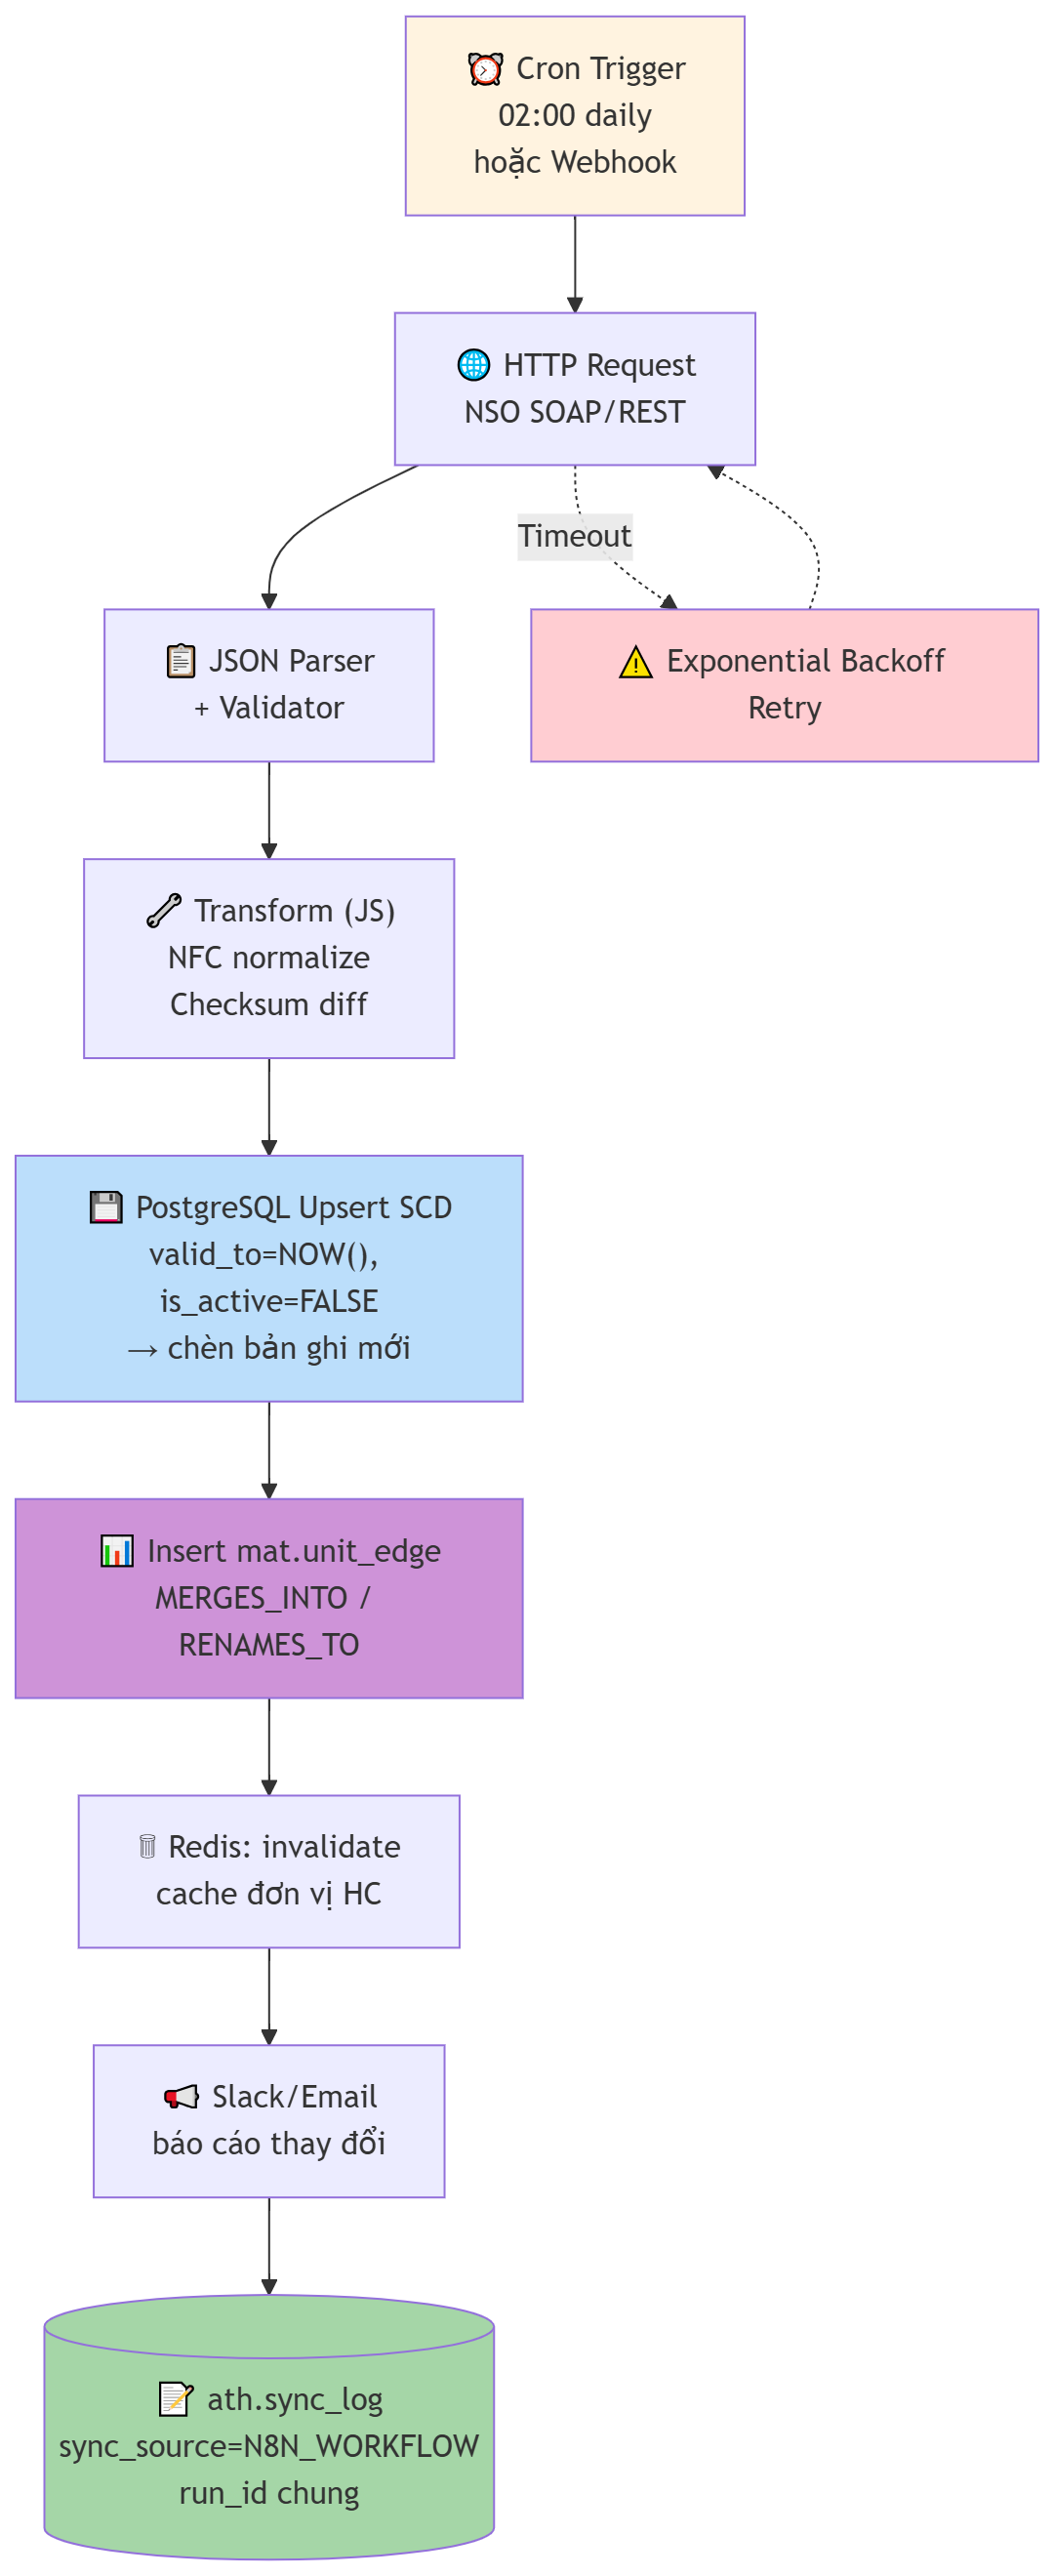
\includegraphics[width=0.3\linewidth]{figs/fig-4-4.png}
% \fbox{\begin{minipage}{0.92\linewidth}\centering\vspace{1.4cm}\textit{[Hình 4.x: Luồng đồng bộ Gov-Sync với n8n. Sáu node tuần tự: \textbf{(1) Cron Trigger} — kích hoạt định kỳ (ví dụ hàng ngày 02:00) hoặc Webhook từ Cổng Chính phủ. \textbf{(2) HTTP Request} — gọi SOAP/REST API NSO lấy danh sách tỉnh/huyện/xã. \textbf{(3) JSON Parser + Validator} — kiểm tra schema phản hồi. \textbf{(4) Transform Node (JavaScript)} — chuẩn hoá Unicode NFC, dịch \texttt{type\_name\_en}, so checksum với master. \textbf{(5) PostgreSQL Upsert SCD} — đóng bản ghi cũ (\texttt{valid\_to = NOW()}, \texttt{is\_active = FALSE}) và chèn bản ghi mới (\texttt{admin\_version = 2}); ghi cạnh vào \texttt{unit\_edge}. \textbf{(6) Notification + Cache Invalidate} — Redis xoá cache đơn vị + gửi Slack/Email báo cáo thay đổi. Mỗi node có nhánh xử lý lỗi với exponential backoff; tất cả ghi vào \texttt{ath.sync\_log} với \texttt{run\_id} chung.]}\vspace{1.4cm}\end{minipage}}
\caption{Luồng đồng bộ Gov-Sync sáu bước với nền tảng n8n.}
\label{fig:gov-sync-workflow}
\end{figure}

\subsection{Chuyển đổi địa chỉ theo kỷ nguyên hành chính}
\label{sec:epoch-migration}

Endpoint \macode{POST /api/migrate-address} là một thành phần phụ trợ nghiên cứu cho phép gửi một chuỗi địa chỉ tự nhiên và nhận kết quả chuyển đổi. Pipeline xử lý gồm ba bước: (1) \macode{EpochDetector} phân loại chuỗi thành PRE\_2025, POST\_2025 hoặc AMBIGUOUS dựa trên các từ khóa đặc trưng (sự xuất hiện của tên đơn vị cũ, từ "Quận" trong khu vực đã chuyển sang "Phường"); (2) nếu phân loại là PRE\_2025, áp dụng bảng \macode{ward\_mapping} để tìm đơn vị hậu cải cách tương ứng; (3) \macode{ACSCalculator} tính điểm tin cậy ACS với \macode{admin\_version} phù hợp.

% ---------------------------------------------------------------------
\section{Module 2: Pipeline AI chuẩn hóa địa chỉ}
\label{sec:ai-pipeline}

\subsection{Lớp tiền xử lý và PreLabeler}
\label{sec:prelabeler}

Lớp tiền xử lý thực hiện bốn nhóm thao tác trên chuỗi đầu vào trước khi đưa vào mô hình học sâu. Thứ nhất, chuẩn hóa Unicode về dạng NFC để xử lý các trường hợp tổ hợp dấu phụ (NFD) phổ biến trên dữ liệu từ iOS/macOS. Thứ hai, chuẩn hóa từ viết tắt theo từ điển 200+ entry phổ biến phân biệt ngữ cảnh Bắc/Nam (ví dụ: "Q." $\to$ "Quận", "P." $\to$ "Phường", "HN" $\to$ "Hà Nội", "TpHCM" $\to$ "Thành phố Hồ Chí Minh"). Thứ ba, loại bỏ thông tin giao hàng (delivery note): các cụm như "gọi trước khi giao", "rẽ phải 150m", "gặp bảo vệ" được tách sang trường \macode{delivery\_instruction} riêng. Thứ tư, chuẩn hóa cấu trúc số nhà/ngõ/ngách: chuỗi "90/12/5" được phân rã thành \{street: 90, alley: 12, house: 5\}.

\textbf{PreLabeler} là engine rule-based kết hợp luật heuristic và từ vựng tiền tố hành chính để sinh nhãn hoặc cấu trúc trung gian. Engine này phục vụ ba mục đích: (i) gán nhãn (annotation) tự động cho dữ liệu huấn luyện ban đầu để giảm chi phí lao động thủ công; (ii) regression testing cho các pattern địa chỉ đã biết; (iii) fallback khi tải mô hình deep learning thất bại --- endpoint phân tích địa chỉ tự động chuyển sang PreLabeler để trả về phản hồi tối thiểu thay vì lỗi 500. Module \macode{address\_cleaner} bổ trợ làm sạch chuỗi đầu vào với các trường hợp cận lề (edge case) phát sinh từ thực tiễn vận hành.

\subsection{Huấn luyện PhoBERT NER}
\label{sec:ner-training}

Script huấn luyện NER thực hiện sáu bước theo trình tự. Bước 1: đọc dữ liệu export từ công cụ gán nhãn Label Studio \cite{LabelStudio2024} hoặc tập Hugging Face công khai. Bước 2: ánh xạ nhãn BIO từ định dạng chuẩn của Label Studio sang lược đồ nhãn dự án --- bảy loại thực thể \{STR (street), WDS (ward), DST (district), PRO (province), HNB (house number), ALY (alley), POI\} với hai nhãn B-/I- cho mỗi loại và một nhãn O, tổng cộng 15 nhãn. Bước 3: tokenize bằng tokenizer PhoBERT (FastBPE) với chiến lược \thuat{label propagation} cho subword: nhãn của từ gốc được nhân rộng cho mọi subword con. Bước 4: huấn luyện \macode{AutoModelForTokenClassification} của Hugging Face Transformers với Trainer; siêu tham số mặc định gồm learning rate 2e-5, batch size 32, 10 epoch, early stopping theo F1 trên tập dev. Bước 5: đánh giá bằng \texttt{seqeval} với ba chỉ số precision, recall, F1 theo chuỗi (sequence-level). Bước 6: ghi lịch sử huấn luyện vào bảng \macode{ath.training\_history} và lưu checkpoint vào thư mục \macode{models/}.

Khung huấn luyện hỗ trợ tăng cường dữ liệu (data augmentation) bằng bốn kỹ thuật: thêm biến thể viết tắt theo từ điển 200+ entry; biến đổi không dấu (loại bỏ ngẫu nhiên dấu thanh và phụ âm trên 20\% mẫu); hoán đổi thứ tự thành phần (ví dụ đảo "Phường X, Quận Y" thành "Quận Y, Phường X"); và thêm nhiễu từ vựng nhẹ (đánh máy sai, lặp ký tự).

\subsection{Retrieval đa tầng với Siamese mGTE}
\label{sec:mgte-retrieval}

Lớp \macode{SiameseMGTE} hiện thực kiến trúc Bi-encoder trên nền checkpoint \path{Alibaba-NLP/gte-}\allowbreak\path{multilingual-base} \cite{mgte2024}. Quy trình ba bước: thứ nhất, mã hóa toàn bộ corpus địa chỉ chuẩn (gộp từ \macode{mat.ward}, \macode{mat.district}, \macode{mat.province}) thành chỉ mục vector kèm metadata (mã GSO, tọa độ centroid, admin\_version) và lưu thành file FAISS. Thứ hai, tại thời điểm truy vấn, mã hóa chuỗi đầu vào (đã chuẩn hóa qua tiền xử lý) thành vector và truy vấn top-k láng giềng gần nhất theo cosine similarity. Thứ ba, lọc kết quả theo \macode{admin\_version} mong muốn và áp dụng kiểm tra phân cấp (Phường $\in$ Quận $\in$ Tỉnh) để loại bỏ các tổ hợp không hợp lệ.

Khi corpus có quy mô lớn (hàng trăm nghìn đơn vị), hệ thống chuyển sang IVF (Inverted File Index) với 1024 cluster và \texttt{nprobe = 16} để duy trì độ trễ dưới 50ms ngay cả khi truy vấn liên tục. Trên API nghiên cứu parser, cấu hình YAML cho phép trỏ tới checkpoint Siamese đã huấn luyện cục bộ thay vì checkpoint mặc định; điều này phục vụ kịch bản fine-tune trên domain địa chỉ Việt Nam như mô tả ở Mục~\ref{sec:siamese}.

\subsection{Tinh chỉnh cấu trúc bằng LLM Qwen}
\label{sec:llm-qwen}

Lớp \macode{LLMQwen3} bọc tokenizer và mô hình causal LM họ Qwen \cite{QwenTeam2024}, được kích hoạt khi điểm tin cậy ACS sau giai đoạn retrieval và NER thấp hơn ngưỡng (mặc định 0.7). Cấu hình thực nghiệm hiện tại sử dụng checkpoint \texttt{Qwen/Qwen2.5-1.5B-Instruct} với lượng tử hóa 4-bit qua BitsAndBytes \cite{Dettmers2022BNB}, temperature 0 cho giải mã tham lam (Greedy Decoding) ổn định. Lựa chọn mô hình 1.5B (thay vì các biến thể lớn hơn 7B/14B) phản ánh sự cân bằng thực tiễn giữa độ chính xác và yêu cầu hạ tầng: 1.5B có thể chạy trên một GPU tiêu dùng (8GB VRAM) sau quantization, đảm bảo tính khả thi triển khai cho doanh nghiệp Việt Nam quy mô vừa.

Prompt được thiết kế theo nguyên tắc \emph{Structured Prompting} với hai thành phần: (i) phần hệ thống mô tả vai trò ``trợ lý chuẩn hóa địa chỉ Việt Nam'' và liệt kê các quy tắc nghiệp vụ (chuẩn 3 cấp Tỉnh--Huyện--Xã, định dạng số nhà); (ii) phần người dùng cung cấp chuỗi đầu vào kèm danh sách top-k ứng viên từ giai đoạn retrieval (Mục~\ref{sec:mgte-retrieval}). Đầu ra yêu cầu định dạng JSON với năm trường: \macode{street}, \macode{ward}, \macode{district}, \macode{province}, \macode{full\_address}. Áp dụng kỹ thuật Constrained Decoding (hoặc parsing nghiêm ngặt) đảm bảo đầu ra luôn hợp lệ về cú pháp JSON.

\subsection{Pipeline production HYBRID\_V1}
\label{sec:hybrid-v1}

Pipeline production tích hợp tất cả thành phần trên thành luồng xử lý tám bước, được kích hoạt trên các bản ghi của \macode{prq.address\_cleansing\_queue} ở trạng thái PENDING hoặc chưa có \macode{address\_standardized}. \cref{tab:hybrid-v1} mô tả chi tiết tám bước.

\begin{table}[H]
\centering
\caption{Tám bước của pipeline production HYBRID\_V1}
\label{tab:hybrid-v1}
\small
\begin{tabularx}{\linewidth}{>{\raggedright\arraybackslash}p{0.6cm} >{\raggedright\arraybackslash}p{3.6cm} >{\raggedright\arraybackslash}X}
\toprule
\textbf{\#} & \textbf{Bước} & \textbf{Mô tả} \\
\midrule
1 & Trích thực thể & \macode{AddressNER} (PhoBERT+BiLSTM-CRF) bóc tách số nhà, đường, ngõ, hành chính \\
2 & Chuẩn hóa tiền tố & Áp dụng map viết tắt cho tên đường (nếu có) \\
3 & Dựng ngữ cảnh & Ghép số nhà, đường, ngõ, các trường hành chính có sẵn trên bản ghi \\
4 & Retrieve top-k & \macode{SiameseMGTE} trả về k ứng viên kèm metadata (tọa độ, GSO ID) \\
5 & LLM refinement & \macode{LLMQwen3} sinh JSON chuẩn hóa từ danh sách ứng viên \\
6 & Detect epoch & \macode{EpochDetector} phân loại PRE\_2025 / POST\_2025 / AMBIGUOUS \\
7 & Tính ACS & Điểm ngữ nghĩa $S_{\text{sem}} = \max(\text{LLM\_score}, \text{Retrieval\_score})$ \\
8 & Ghi kết quả & Cập nhật \macode{address\_standardized}, ACS, \macode{processing\_method='HYBRID\_V1'}; back-fill lat/lng từ metadata top-1 nếu thiếu \\
\bottomrule
\end{tabularx}
\end{table}

Việc lấy $\max$ giữa điểm LLM và điểm retrieval tại bước 7 phản ánh nguyên tắc \emph{lạc quan thận trọng (cautious optimism)}: nếu một trong hai mô hình đưa ra điểm cao đáng tin cậy thì hệ thống tin theo, nhưng cờ \macode{selected\_ai\_model} ghi lại nguồn quyết định để hỗ trợ phân tích lỗi và truy vết về sau. \cref{fig:hybrid-v1-pipeline} thể hiện trực quan toàn bộ pipeline tám bước.

\begin{figure}[H]
\centering
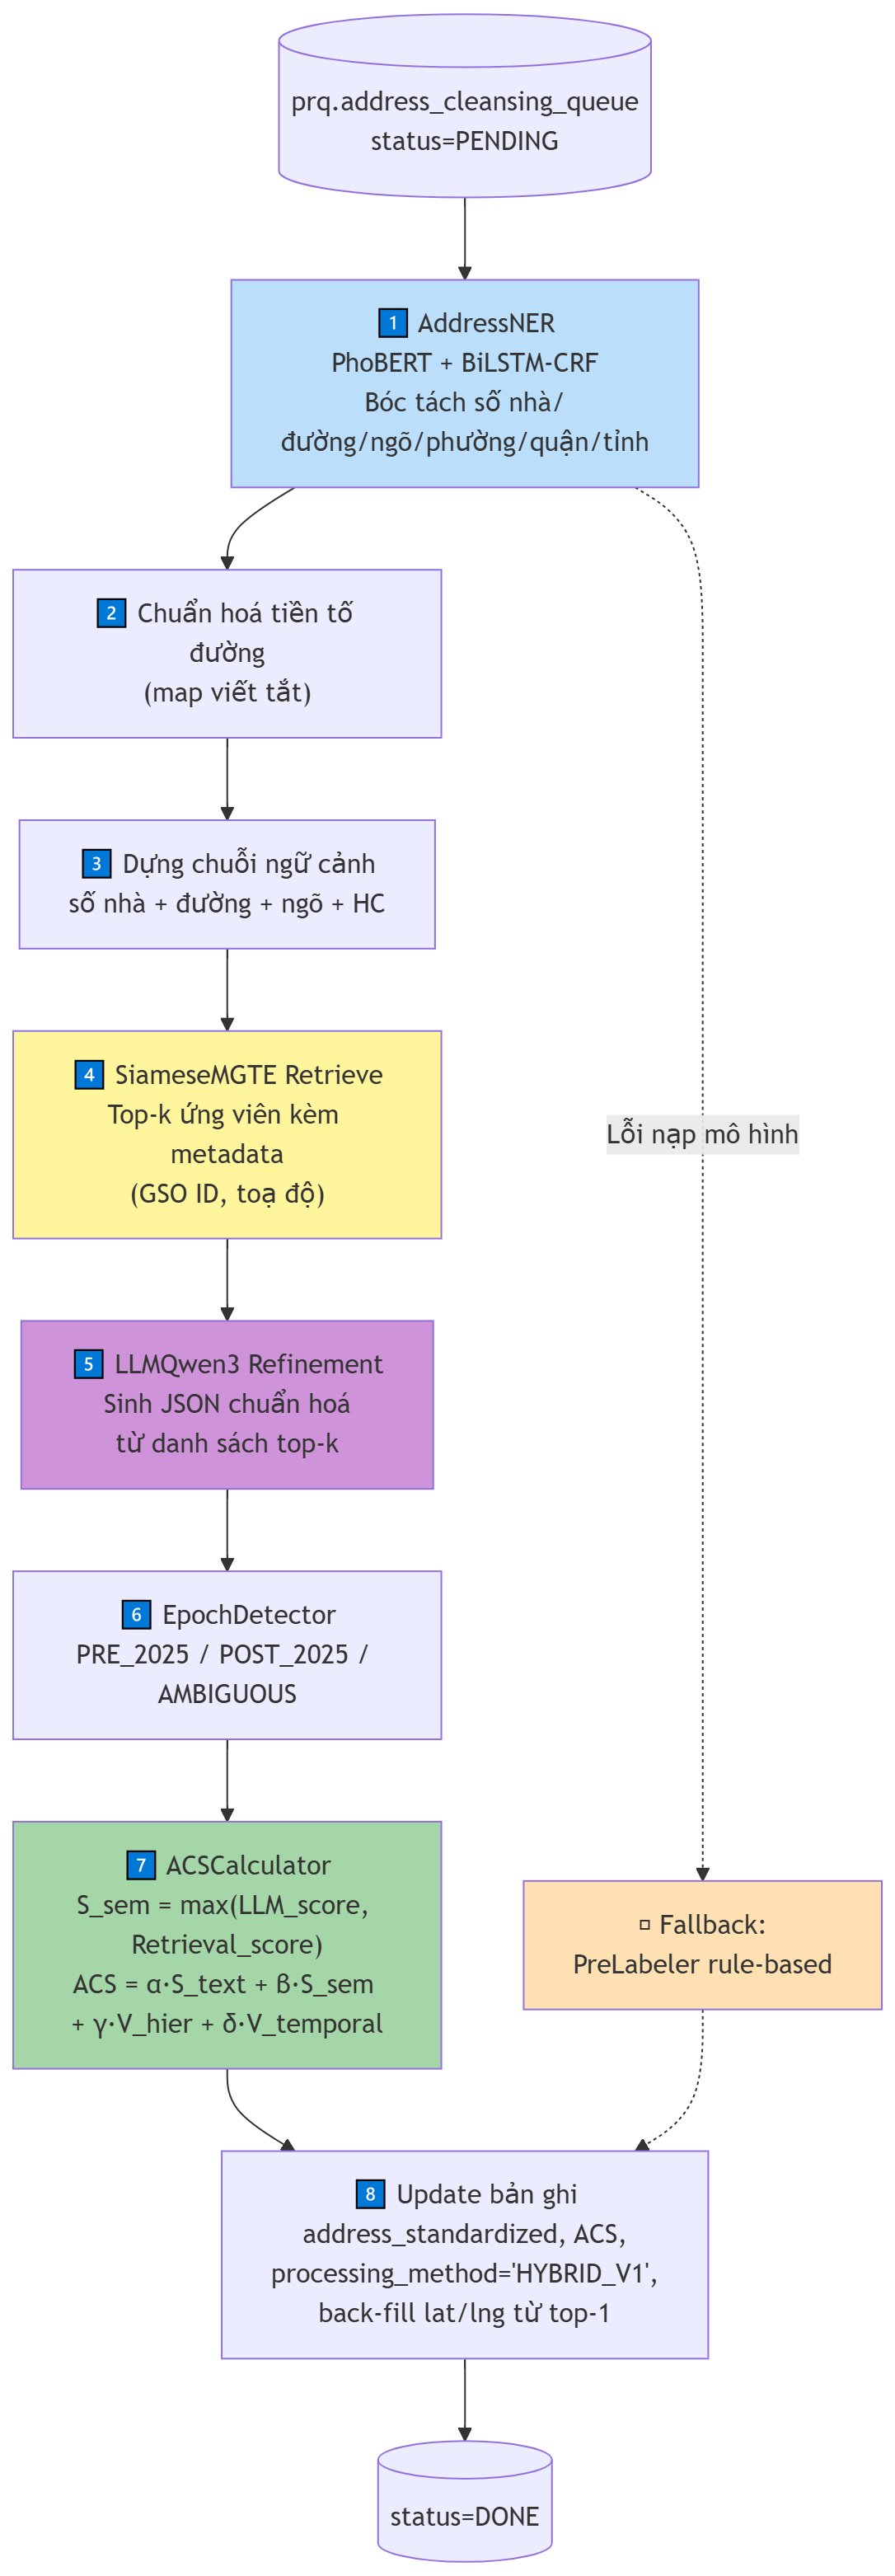
\includegraphics[width=0.4\linewidth]{figs/fig-4-5.png}
% \fbox{\begin{minipage}{0.92\linewidth}\centering\vspace{1.4cm}\textit{[Hình 4.x: Sơ đồ pipeline production HYBRID\_V1 tám bước. \textbf{Đầu vào}: bản ghi \texttt{prq.address\_cleansing\_queue} ở trạng thái PENDING. \textbf{Bước 1}: AddressNER (PhoBERT+BiLSTM-CRF) bóc tách số nhà, đường, ngõ, phường, quận, tỉnh. \textbf{Bước 2}: chuẩn hoá tiền tố đường theo map viết tắt. \textbf{Bước 3}: dựng chuỗi ngữ cảnh từ NER + trường khai báo. \textbf{Bước 4}: SiameseMGTE retrieve top-$k$ ứng viên từ FAISS index. \textbf{Bước 5}: LLMQwen3 sinh JSON chuẩn hoá từ danh sách top-$k$. \textbf{Bước 6}: EpochDetector phân loại PRE\_2025 / POST\_2025 / AMBIGUOUS. \textbf{Bước 7}: ACSCalculator tính điểm với $S_{\text{sem}} = \max(\text{LLM\_score}, \text{Retrieval\_score})$. \textbf{Bước 8}: cập nhật \texttt{address\_standardized}, ACS, \texttt{processing\_method='HYBRID\_V1'}, back-fill lat/lng. Các nhánh fallback đến PreLabeler khi mô hình thất bại được vẽ bằng đường đứt.]}\vspace{1.4cm}\end{minipage}}
\caption{Pipeline production HYBRID\_V1 tám bước.}
\label{fig:hybrid-v1-pipeline}
\end{figure}

\subsection{So sánh đa mô hình trên API nghiên cứu}
\label{sec:multi-model}

Endpoint \macode{POST /api/parser/analyze} cho phép client gửi một chuỗi địa chỉ và nhận về kết quả phân tích từ bốn mô hình chạy song song: \macode{AddressNER}, \macode{PhoBERTSiamese} (backbone \texttt{vinai/phobert-base}), \macode{SiameseMGTE}, và \macode{LLMQwen3}. Sau đó, nếu import thành công, ACS và epoch được tính trên cơ sở điểm số tốt nhất trong các đầu ra có trường score. Endpoint \macode{GET /api/parser/status} và \macode{POST /api/parser/reload} hỗ trợ vận hành theo dõi lỗi nạp GPU/CPU và nạp lại checkpoint mà không cần restart toàn bộ server.

\subsection{Pipeline huấn luyện liên tục từ PreLabeler Cases}
\label{sec:continuous-training}

Khung giải pháp hỗ trợ huấn luyện lại PhoBERT NER từ các mẫu PreLabeler đã được con người xác nhận đạt chuẩn, đóng vòng phản hồi (\thuat{feedback loop}) giữa người dùng và mô hình. Cơ chế gồm bốn cấu phần.

\emph{Cấu phần 1 --- Nguồn dữ liệu.} Schema \macode{ai.prelabeler\_testcases} lưu các bản ghi gán nhãn với cấu trúc \macode{input} JSONB (chuỗi địa chỉ thô), \macode{expected} JSONB (danh sách thực thể kỳ vọng), \macode{test\_result} JSONB (kết quả validation), \macode{strict} BOOLEAN. Chỉ các mẫu có \macode{test\_result->>'passed' = true} mới được đưa vào tập huấn luyện, đảm bảo dữ liệu đầu vào đã qua kiểm tra validation hai chiều (expected entities phải có mặt; không có unexpected entities nếu strict mode).

\emph{Cấu phần 2 --- Endpoint kích hoạt.} Endpoint\\ \macode{POST /api/training/trigger-ner-from-prelabeler} (yêu cầu xác thực) kiểm tra số lượng mẫu đạt chuẩn; nếu vượt ngưỡng tối thiểu (mặc định 50 mẫu), hệ thống \thuat{spawn} tiến trình nền chạy \macode{train\_ner.py} với cờ \macode{--from-prelabeler}.

\emph{Cấu phần 3 --- Chuyển đổi định dạng.} Hàm \macode{\_prelabeler\_case\_to\_labelstudio()} tính \thuat{character offset} của từng thực thể trong chuỗi gốc bằng so khớp chuỗi, tạo cấu trúc annotation tương đương Label Studio. Hàm \macode{convert\_labelstudio\_to\_bio()} đã có sẵn xử lý tokenization và gán nhãn BIO cho từng sub-token PhoBERT. Tham số \macode{--merge-labelstudio} cho phép kết hợp với export từ Label Studio (file \macode{data/labeled\_export.json}) để mở rộng quy mô tập huấn luyện và đa dạng hoá miền dữ liệu.

\emph{Cấu phần 4 --- Quản lý phiên bản và provenance.} Mỗi lần huấn luyện tạo thư mục checkpoint mới theo quy ước \macode{models/phobert-ner-vn-YYYYMMDD-HHMMSS/}, chứa trọng số mô hình, tokenizer config và file \macode{training\_log.json} ghi nhận siêu tham số, nguồn dữ liệu (số mẫu prelabeler, số mẫu Label Studio nếu merge), chỉ số F1/precision/recall/token accuracy trên tập kiểm định, và git commit hash. Metadata được ghi đồng thời vào \macode{ath.training\_history} qua hàm \macode{record\_training\_history()} với trường \macode{notes} chứa chuỗi mô tả đầy đủ dạng \\ \texttt{prelabeler\_cases=120; labelstudio\_merged=0; epochs=10; batch\_size=16; lr=2e-5; eval\_split=0.2; eval\_loss=0.1573}; cấu trúc này cho phép tái lập chính xác điều kiện thực nghiệm khi cần đối chiếu hoặc rollback checkpoint.

% ---------------------------------------------------------------------
\section{Module 3: Geospatial và hiệu chỉnh polygon}
\label{sec:geospatial}

\subsection{Thu thập OpenStreetMap}
\label{sec:osm-collection}

CLI và REST API hỗ trợ kích hoạt job thu thập OSM qua client \texttt{overpy} gọi Overpass API \cite{OSM2024Overpass} công khai. Job nhận hai tham số: phạm vi địa lý (giới hạn theo \macode{province\_id}) và mục tiêu tổng số thực thể. Trạng thái job được giữ trong biến tiến trình toàn cục có khóa mutex để đảm bảo không có hai job chạy đồng thời trên cùng phạm vi. Sau khi tải về, dữ liệu thô được phân tích cú pháp và phân loại vào ba bảng \macode{osm.streets}, \macode{osm.buildings}, \macode{osm.pois} dựa trên các tag OSM gốc; bản ghi thô được lưu vào \macode{osm.raw\_entities}. Endpoint \macode{GET /api/osm/summary} và \macode{/preview} phục vụ dashboard quan sát tiến trình thu thập.

\subsection{Lưu trữ polygon và trực quan hóa ranh giới}
\label{sec:polygon-storage}

Bảng \macode{mat.area\_polygon} lưu ranh giới đơn vị hành chính dưới dạng GeoJSON. API \url{GET /api/boundary/map} nhận tham số \macode{level} và \macode{unit\_id}, tạo bản đồ Folium \cite{Folium2024} hiển thị polygon trên nền OpenStreetMap, trả về đường dẫn file HTML có thể nhúng vào dashboard hoặc gửi tới người dùng cuối. Trường hợp polygon không tồn tại (đơn vị hành chính mới được tạo mà chưa có dữ liệu OSM), hệ thống trả về bản đồ rỗng với cảnh báo thay vì lỗi cứng, đảm bảo trải nghiệm người dùng nhất quán.

Để hỗ trợ phân tích trực quan, công cụ \macode{tools/boundary\_visualization} cho phép xuất bản đồ HTML đa lớp gom polygon theo nhiều cấp hành chính, dùng cho debug và viết case study.

\subsection{API spatial: Point-in-Polygon và Mismatch Report}
\label{sec:spatial-api}

Endpoint \macode{POST /api/spatial/subdivide} nhận danh sách điểm (lat, lng) cùng \macode{level} $\in$ \{province, district, ward\} và trả về phân nhóm đơn vị hành chính tương ứng. Logic xử lý hai tầng: nếu PostGIS extension đã được cài đặt, hệ thống thử \macode{ST\_Contains} giữa điểm và geometry chuyển từ GeoJSON; nếu không có match (điểm nằm sát ngoài biên do sai số GPS), fallback sang \macode{ST\_Distance} tới centroid để chọn đơn vị gần nhất. Phản hồi gồm bốn nhóm thống kê: số điểm khớp polygon, số điểm khớp theo nearest, số điểm không khớp, và cờ \macode{postgis\_available}.

Endpoint \macode{GET /api/spatial/mismatch-report} thực hiện so khớp giữa \\ \macode{\path{prq.address_cleansing_queue}} (chứa lat/lng đã làm giàu) và polygon cấp ward: tìm các bản ghi có tọa độ nằm trong polygon của ward khác với \macode{ward\_id} đã khai báo. Truy vấn có thể lọc theo \macode{province\_id} và giới hạn số lượng kết quả. Kết quả này là đầu vào cốt lõi cho quy trình hiệu chỉnh polygon mô tả ở mục tiếp theo.

\subsection{Edge Injection cho hiệu chỉnh GPS gần biên}
\label{sec:edge-inject}

Hàm \macode{edge\_inject\_lookup} hiện thực chiến lược thứ ba trong ba chiến lược hiệu chỉnh polygon đã trình bày ở Chương 3, Mục 3.6.5. Cụ thể, khi một tọa độ GPS được phát hiện nằm sát biên giữa hai đơn vị hành chính kề nhau, hàm thực hiện bốn bước: thứ nhất, truy vấn \macode{mat.unit\_edge} để lấy danh sách các đơn vị láng giềng (qua các cạnh kiểu \macode{BOUNDARY\_ADJUSTED}); thứ hai, tính khoảng cách Haversine từ điểm cần kiểm tra tới centroid của từng đơn vị láng giềng (hoặc qua polygon nếu bảng không lưu centroid trực tiếp cho cấp đó); thứ ba, lọc các đơn vị có khoảng cách dưới ngưỡng bán kính (mặc định 200m, cấu hình được); thứ tư, chọn đơn vị có khoảng cách nhỏ nhất và đề xuất gán điểm cho đơn vị đó.

Mục đích của Edge Injection là giảm lỗi gán đơn vị khi điểm GPS rơi sát ranh giới do sai số GPS (thường 5--15m trên thiết bị di động) hoặc nhiễu địa lý. Kết quả của hàm này được tích hợp vào pipeline HYBRID\_V1 (Mục~\ref{sec:hybrid-v1}) như một bước hậu xử lý cho các bản ghi có \macode{phobert\_confidence\_score} cao nhưng đối soát không gian thất bại.

Module \macode{geometry/buffer\_union} và \macode{geometry/concave\_hull} hiện thực hai chiến lược còn lại (Buffer-Union và Concave Hull/Alpha Shape) dựa trên thư viện Shapely \cite{Shapely2024} và alphashape, cho phép mở rộng polygon hoặc tái dựng biên từ đám mây điểm giao nhận thực tế.

% ---------------------------------------------------------------------
\section{Module 4: Làm giàu dữ liệu đa nguồn}
\label{sec:enrichment}

\subsection{Chiến lược thu thập đa nguồn và Waterfall Enrichment}
\label{sec:waterfall}

Module làm giàu tuân theo kiến trúc Waterfall Enrichment đã đề xuất trong dàn ý nghiên cứu: ba lớp xếp tầng theo thứ tự ưu tiên chi phí thấp $\to$ chi phí cao. Lớp 1 (Internal Cache Redis): chi phí 0, hit rate kỳ vọng 20--40\% với các địa chỉ phổ biến đã xử lý trước đó. Lớp 2 (OSM + VietMap): chi phí thấp, độ trễ thấp do server đặt tại Việt Nam, độ phủ ước tính 40--50\% các địa chỉ. Lớp 3 (Google Maps Geocoding API): chỉ kích hoạt khi confidence thấp, mục tiêu giới hạn dưới 10--20\% tổng số request để kiểm soát chi phí. \cref{fig:waterfall-enrichment} minh hoạ kiến trúc thác nước và tỷ lệ phân bổ giữa các lớp.

\begin{figure}[H]
\centering
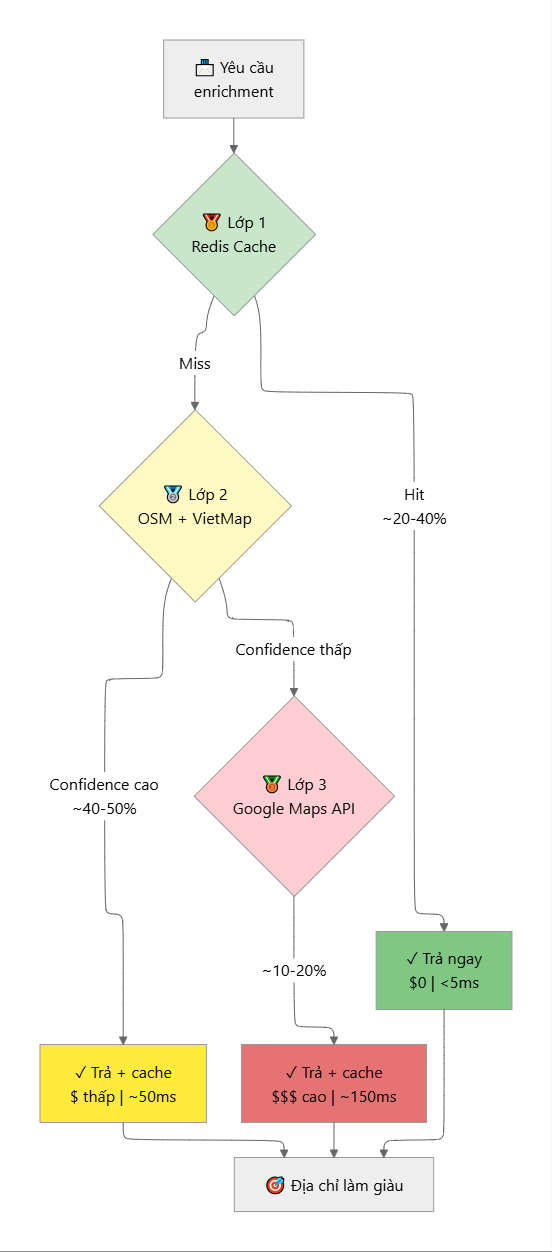
\includegraphics[width=0.4\linewidth]{figs/fig-4-6.png}
% \fbox{\begin{minipage}{0.92\linewidth}\centering\vspace{1.4cm}\textit{[Hình 4.x: Kiến trúc Waterfall Enrichment ba lớp. Hình vẽ dạng phễu lật ngược từ trái sang phải: \textbf{Lớp 1 (Cache Redis, miễn phí)} chiếm $\sim$ 20--40\% lưu lượng → các yêu cầu không hit Cache rơi xuống. \textbf{Lớp 2 (OSM + VietMap, chi phí thấp)} chiếm $\sim$ 40--50\% → các yêu cầu confidence thấp rơi xuống. \textbf{Lớp 3 (Google Maps API, chi phí cao)} chỉ $\sim$ 10--20\% → đảm bảo độ phủ tổng thể $\geq 95\%$. Bên dưới mỗi lớp ghi rõ độ trễ trung bình kỳ vọng (ms) và chi phí mỗi 1.000 request. Mũi tên xuống thể hiện luồng fallback; mũi tên ngang trên cùng thể hiện hit cache tránh fallback.]}\vspace{1.4cm}\end{minipage}}
\caption{Kiến trúc Waterfall Enrichment ba lớp Cache--OSM/VietMap--Google.}
\label{fig:waterfall-enrichment}
\end{figure}

Cụ thể, bốn nguồn dữ liệu chính trong module enrichment được tổng hợp tại \cref{tab:enrichment-sources}.

\begin{table}[H]
\centering
\caption{Bốn nguồn dữ liệu trong module làm giàu}
\label{tab:enrichment-sources}
\small
\begin{tabularx}{\linewidth}{>{\raggedright\arraybackslash}p{3cm} >{\raggedright\arraybackslash}p{3.4cm} >{\raggedright\arraybackslash}X}
\toprule
\textbf{Nguồn} & \textbf{Loại dữ liệu} & \textbf{Vai trò trong VNAI} \\
\midrule
NSO (Government) & Danh mục hành chính chính thức & Cập nhật \schema{mat}, mã GSO, ranh giới hành chính \\
OpenStreetMap   & Đường, tòa nhà, POI       & Làm giàu \schema{osm}; bounding box theo đơn vị \\
Google Maps     & Tọa độ chính xác, POI thương mại & Fallback khi OSM thiếu dữ liệu \\
VietMap         & Migration address, POI Việt & Xử lý vùng nông thôn (đề xuất tích hợp tương lai) \\
\bottomrule
\end{tabularx}
\end{table}

\subsection{Bộ nhớ đệm Redis và xóa cache có chọn lọc}
\label{sec:redis-cache}

Lớp 1 của Waterfall Enrichment được hiện thực bằng Redis \cite{Redis2024}. Cache có hai chế độ hoạt động. Chế độ \emph{lookup cache}: lưu kết quả các truy vấn enrichment theo khóa hash của địa chỉ chuẩn hóa, TTL 7 ngày. Chế độ \emph{admin unit cache}: lưu toàn bộ danh mục đơn vị hành chính active để giảm truy vấn DB cho các endpoint \macode{/provinces}, \macode{/districts}, \macode{/wards}; cache này được tự động invalidate khi sync NSO ghi nhận thay đổi.

Hai endpoint quản trị được cung cấp: \macode{GET /api/cache/health} kiểm tra sức khỏe kết nối Redis; \macode{DELETE /api/cache/admin} xóa cache đơn vị hành chính (yêu cầu xác thực, dùng sau khi sync NSO thủ công).

\subsection{Provenance và quản lý nguồn gốc dữ liệu}
\label{sec:provenance}

Mọi bản ghi địa chỉ và đơn vị hành chính trong VNAI đều mang thông tin provenance dưới dạng cột \macode{source}, \macode{source\_system} hoặc tương đương: \macode{mat.area\_polygon.source} $\in$ \{OSM, GSO, MANUAL\}; \macode{prq.ground\_truth.source\_system} $\in$ \{TYPESENSE, GOOGLE, MANUAL\}. Cách thiết kế này cho phép truy vết nguồn gốc cho mọi quyết định của hệ thống, hỗ trợ phân tích lỗi và audit dữ liệu trong trường hợp có khiếu nại.

Đặc biệt, mọi run đồng bộ ground truth từ Typesense được ghi vào \\ \macode{ath.typesense\_ground\_truth\_sync\_run} với các trường \macode{started\_at}, \macode{finished\_at}, \macode{records\_scanned}, \macode{records\_upserted}. Liên kết khóa ngoại từ\\ \macode{prq.ground\_truth.last\_sync\_run\_id} đến bảng run này tạo thành dấu vết kiểm tra (audit trail) đầy đủ.

% ---------------------------------------------------------------------
\section{Tầng API REST và giao diện người dùng}
\label{sec:api-ui}

\subsection{Kiến trúc client SPA}
\label{sec:spa}

Giao diện người dùng được hiện thực dưới dạng Single Page Application (SPA) nhẹ với HTML/CSS/JavaScript thuần (không sử dụng framework như React/Vue). Quyết định này phản ánh hai ưu tiên: thứ nhất, giảm độ phức tạp triển khai cho doanh nghiệp quy mô vừa (không cần build pipeline Node.js); thứ hai, đảm bảo khả năng tích hợp dễ dàng với các backoffice hiện hữu của doanh nghiệp.

Logic client gồm bốn lớp. Thứ nhất, lớp xác thực: kiểm tra JSON Web Token (JWT) trong \macode{sessionStorage}; nếu thiếu và không ở trang đăng nhập thì chuyển hướng tự động. Thứ hai, lớp fetch: hàm \macode{apiFetch} thử nhiều base URL API theo thứ tự (localhost cho dev, origin hiện tại cho production, cấu hình người dùng cho deployment đặc biệt). Thứ ba, lớp điều hướng: shell điều hướng theo thuộc tính HTML \macode{data-page}, mỗi trang con tương ứng một màn chức năng. Thứ tư, lớp giao diện: cho phép đổi theme (\macode{dark}, \macode{light}, \macode{oled-black}) và chế độ chuyển động (\macode{prefers-reduced-motion}).

Các chức năng được tổ chức thành ba nhóm: nhóm vận hành (\thuat{overview}, \thuat{parser}, \thuat{batch}, \thuat{explorer}, \thuat{lookup}); nhóm nghiên cứu (\thuat{training}, \thuat{experiments}, \thuat{evidence}, \thuat{label-registry}, \thuat{prelabeler-cases}, \thuat{label-studio}); nhóm dữ liệu (\thuat{admin-units}, \thuat{nso-sync}, \thuat{osm-enrichment}, \thuat{boundary-visualization}, \thuat{documentation}).

\subsection{Phân nhóm endpoint REST}
\label{sec:rest-grouping}

Toàn bộ API được tổ chức thành sáu nhóm endpoint theo tiền tố URL. Nhóm chính \macode{/api/*} chứa các endpoint cốt lõi; router phiên bản \macode{/api/v1/*} mirror cùng tập endpoint nhằm hỗ trợ phiên bản hóa API trong tương lai. Bốn nhóm con thuộc các module chuyên biệt: \macode{/api/spatial/*} cho geospatial, \macode{/api/boundary/*} cho ranh giới, \macode{/api/repo-docs/*} cho đọc tài liệu kho mã (chỉ trong thư mục \macode{docs/}, loại trừ nhánh private), và các endpoint xác thực không gắn tiền tố module.

\cref{tab:rest-endpoints} liệt kê các endpoint cốt lõi theo nhóm chức năng nghiệp vụ.

\begin{table}[H]
\centering
\caption{Các endpoint REST cốt lõi theo nhóm chức năng}
\label{tab:rest-endpoints}
\small
\begin{tabularx}{\linewidth}{>{\raggedright\arraybackslash}p{2.6cm} >{\raggedright\arraybackslash}X}
\toprule
\textbf{Nhóm} & \textbf{Endpoint (method và đường dẫn sau /api)} \\
\midrule
Xác thực     & \macode{POST /login}, \macode{/register/send-code}, \macode{/register}, \macode{/logout} \\
Tra cứu HC   & \macode{GET /provinces}, \macode{/districts/\{province\_id\}}, \macode{/wards/\{district\_id\}}, \macode{/unit-details/\{level\}/\{unit\_id\}}, \macode{/lookup/mapping} \\
Đồng bộ NSO & \macode{POST /sync/nso}, \macode{/sync/nso/province}; \macode{GET /sync/nso/logs}; \macode{GET /nso/\{provinces|districts|wards\}} \\
AI Parser   & \macode{GET /parser/status}, \macode{/parser/sample}; \macode{POST /parser/reload}, \macode{/parser/analyze}; \macode{POST /migrate-address} \\
Hàng đợi    & \macode{GET /queue/summary}, \macode{/explorer/queue}; \macode{POST /batch/trigger}; \macode{GET /batch/job} \\
Huấn luyện  & \macode{GET /training/history}, \macode{/training/samples}; \macode{POST /training/history} \\
Benchmark   & \macode{GET /benchmark/realtime}, \macode{/benchmark/baselines}, \macode{/benchmark/job}; \macode{POST /benchmark/trigger} \\
OSM         & \macode{GET /osm/\{summary|preview|job\}}; \macode{POST /osm/trigger} \\
Spatial     & \macode{POST /api/spatial/subdivide}; \macode{GET /api/spatial/\{mismatch-report|postgis-status\}} \\
Boundary    & \macode{GET /api/boundary/map} \\
Lịch sử HC  & \macode{GET /admin-unit/\{level\}/\{unit\_id\}/history}; \macode{/sync-logs}, \macode{/sync-logs/summary/\{run\_id\}} \\
PreLabeler  & \macode{GET /prelabeler-cases}, \macode{/random-predict}; \macode{POST /prelabeler-cases}, \macode{/run}, \macode{/export-label-studio} \\
Cache       & \macode{GET /cache/health}; \macode{DELETE /cache/admin} \\
\bottomrule
\end{tabularx}
\end{table}

\subsection{Xác thực JWT và bảo mật}
\label{sec:jwt}

Hệ thống sử dụng JSON Web Token (JWT) cho xác thực phiên người dùng. Luồng đăng ký yêu cầu xác thực email hai bước: \macode{POST /register/send-code} gửi mã 6 chữ số tới email, lưu vào \macode{ath.email\_verifications} với TTL 15 phút; \macode{POST /register} hoàn tất với mã đã nhận. Mật khẩu được hash bằng bcrypt qua thư viện \texttt{passlib}. Token JWT có thời hạn cấu hình được (mặc định 60 phút) và được kiểm tra trên các endpoint nghiệp vụ thông qua dependency \macode{get\_current\_user} của FastAPI. Một số endpoint trigger (batch, OSM, cache delete) yêu cầu xác thực để ngăn việc kích hoạt trái phép từ bên ngoài.

% ---------------------------------------------------------------------
\section{Khung thực nghiệm SUPA-Bench}
\label{sec:supa}

\subsection{Định nghĩa và mục tiêu}
\label{sec:supa-definition}

SUPA-Bench (\textit{Synthetic User-style Perturbation Address benchmark}) là khung đánh giá chuẩn hóa địa chỉ được thiết kế chuyên biệt cho bối cảnh dữ liệu lưỡng thời của Việt Nam. Khác với các benchmark NER truyền thống vốn đo lường độ chính xác trên dữ liệu sạch đã gán nhãn, SUPA-Bench mô phỏng cách người dùng thực tế gõ địa chỉ với nhiễu (perturbation) theo các pattern phổ biến, đồng thời cho phép đánh giá Exact Match (EM) song song với cả hai phiên bản tham chiếu (hậu cải cách v2 và tiền cải cách v1).

Mục tiêu cốt lõi của SUPA-Bench là cung cấp một khung tái lập (reproducible) cho mọi thực nghiệm chuẩn hóa địa chỉ trong khung VNAI, đảm bảo các báo cáo khoa học có thể so sánh được giữa các phiên bản mô hình, các checkpoint khác nhau, và các nghiên cứu kế thừa trong tương lai. Bất biến nghiên cứu cốt lõi (đã nêu tại Mục~\ref{sec:supa-tables}) là pipeline SUPA-Bench chỉ đọc \macode{prq.ground\_truth} mà không thực hiện bất kỳ thao tác ghi nào, đảm bảo tính độc lập giữa nguồn tham chiếu và quy trình đánh giá.

\subsection{Quy trình SUPA-Bench năm bước}
\label{sec:supa-workflow}

\cref{tab:supa-steps} mô tả năm bước của quy trình SUPA-Bench, từ chuẩn bị cơ sở dữ liệu đến xuất báo cáo. \cref{fig:supa-workflow} thể hiện trực quan luồng các lệnh CLI cùng các artifact đầu ra.

\begin{figure}[H]
\centering
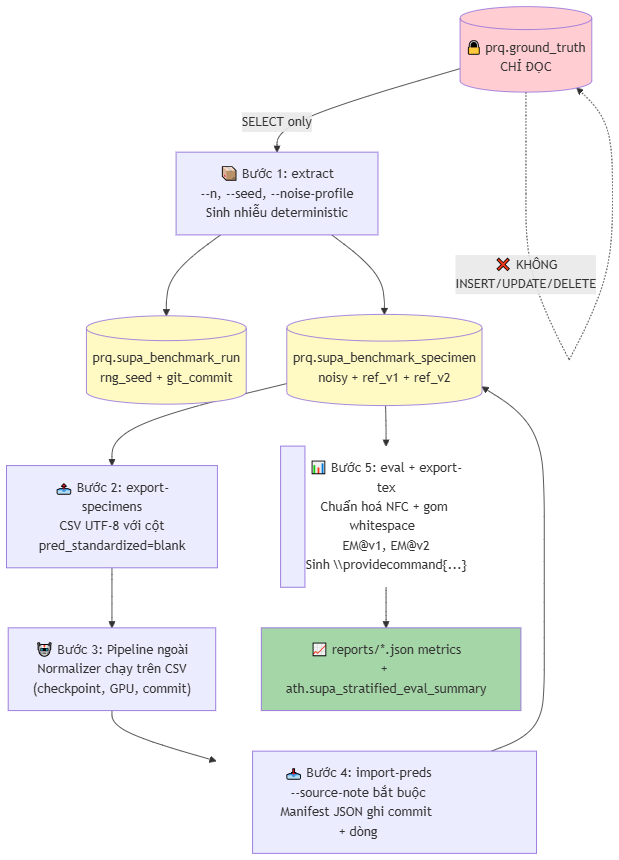
\includegraphics[width=0.5\linewidth]{figs/fig-4-7.png}
% \fbox{\begin{minipage}{0.92\linewidth}\centering\vspace{1.4cm}\textit{[Hình 4.x: Workflow SUPA-Bench năm bước. \textbf{Bước 0 (DDL)}: migration tạo bảng \texttt{prq.supa\_benchmark\_run/specimen}. \textbf{Bước 1 (\texttt{extract})}: SQL \texttt{SELECT} từ \texttt{prq.ground\_truth} (chỉ đọc) + hàm sinh nhiễu deterministic → tạo cohort với \texttt{rng\_seed} ghi vào DB. \textbf{Bước 2 (\texttt{export-specimens})}: xuất CSV với cột \texttt{noisy\_raw\_address}, \texttt{ref\_address\_v1/v2}, cột trống \texttt{pred\_standardized}. \textbf{Bước 3 (Pipeline ngoài)}: chạy normalizer trên CSV; người vận hành kèm \texttt{--source-note}. \textbf{Bước 4 (\texttt{import-preds})}: nhập lại CSV đã điền dự đoán; manifest JSON ghi commit + số dòng. \textbf{Bước 5 (\texttt{eval} + \texttt{export-tex})}: chuẩn hoá NFC + tính EM v1/v2 → JSON metrics → macro LaTeX \texttt{\textbackslash providecommand}. Đường nét đứt thể hiện bất biến: không có thao tác WRITE nào hướng về \texttt{ground\_truth}.]}\vspace{1.4cm}\end{minipage}}
\caption{Workflow SUPA-Bench.}
\label{fig:supa-workflow}
\end{figure}

\begin{table}[H]
\centering
\caption{Năm bước của quy trình SUPA-Bench}
\label{tab:supa-steps}
\small
\begin{tabularx}{\linewidth}{>{\raggedright\arraybackslash}p{0.6cm} >{\raggedright\arraybackslash}p{3cm} >{\raggedright\arraybackslash}X}
\toprule
\textbf{\#} & \textbf{Lệnh con CLI} & \textbf{Mô tả} \\
\midrule
0 & DDL chuẩn bị      & Tạo \macode{prq.supa\_benchmark\_run} và \macode{supa\_benchmark\_specimen} qua migration SQL \\
1 & \macode{extract}  & Chọn cohort từ ground truth, sinh nhiễu deterministic theo seed, ghi specimen \\
2 & \macode{export-specimens} & Xuất CSV UTF-8 với cột \macode{noisy\_raw\_address}, \macode{ref\_address\_v1/v2}, cột trống \macode{pred\_standardized} \\
3 & \macode{import-preds} & Đọc lại CSV sau khi pipeline ngoài chạy dự đoán; bắt buộc \macode{--source-note} \\
4 & \macode{eval}     & Tổng hợp Exact Match v1\% và v2\%; chuẩn hóa NFC + gom whitespace trước so khớp \\
5 & \macode{export-tex} & Sinh \macode{providecommand} cho RunId, cỡ mẫu, EM\%, seed, commit \\
\bottomrule
\end{tabularx}
\end{table}

\textbf{Profile nhiễu SUP-1.0.0 (chuẩn).} Hàm sinh nhiễu deterministic theo \macode{random.Random(seed)} áp năm loại perturbation phổ biến: (i) viết tắt đơn vị hành chính (\texttt{Q.}, \texttt{P.}, \texttt{Đ.}, \texttt{TP.}) với xác suất 65\%; (ii) hoán đổi vùng miền (\texttt{Ngõ} \(\leftrightarrow\) \texttt{Hẻm}, \texttt{Ngách} \(\leftrightarrow\) \texttt{Kiệt}) với xác suất 30\%; (iii) thêm tiền tố vị trí kiểu ``Gần '', ``Đối diện '', ``Bên cạnh '' với xác suất 40\%; (iv) lỗi bộ gõ nhẹ (đ/dd, â/aa, Hoà/Hòa) mô phỏng lỗi gõ IME; (v) biến đổi khoảng trắng (thêm hoặc gấp đôi khoảng trắng nội bộ).

\textbf{Profile nhiễu SUP-D2-1.0.0 (thách thức cao).} Phiên bản tăng cường nhằm kiểm tra độ bền (\thuat{robustness}) của pipeline trên đầu vào cực đoan: (i) \emph{loại bỏ hoàn toàn dấu tiếng Việt} (\thuat{unaccented}); (ii) viết tắt đơn vị hành chính gần như tuyệt đối (90\%); (iii) lỗi ký tự vật lý nâng cao --- hoán đổi (\thuat{transposition}) và lặp ký tự thay vì chỉ lỗi IME; (iv) xác suất tiền tố nâng lên 60\% và hoán đổi vùng miền lên 60\%; (v) xoá khoảng trắng sau dấu phẩy (ví dụ \texttt{Quận 1,TP.HCM}) để gây khó khăn cho bước tokenization. Profile này được sử dụng riêng cho tầng D2 trong cơ cấu cohort phân tầng (\cref{tab:strata}).

Tính chất deterministic của seed (đối với cả hai profile) đảm bảo mọi lần chạy với cùng seed sinh cùng tập specimen, là điều kiện cần cho khả năng tái lập.

\subsection{Lệnh gộp workflow}
\label{sec:supa-workflow-cmd}

Lệnh \macode{workflow} thực hiện chuỗi tự động: \macode{extract} (trừ khi \macode{--skip-extract}) $\to$ \\ \macode{export-specimens} $\to$ \macode{import-preds} (nếu có CSV dự đoán) $\to$ \macode{eval} $\to$ \macode{export-tex}. Tham số \macode{--n} mặc định là 10.000 mẫu; khi chỉ cần cohort nhỏ cho thử nghiệm cần truyền \macode{--n} tường minh. Cờ \macode{--preds-demo-ref-v2} tạo file dự đoán \emph{oracle} bằng cách sao chép \macode{ref\_address\_v2} sang \macode{pred\_standardized}, chỉ phục vụ smoke test đường ống mà không được dùng làm bằng chứng mô hình; cờ \macode{--source-note} bắt buộc khi có \macode{--preds} thực tế.

Đầu ra \macode{export-tex} sinh các macro \macode{providecommand} cho RunId, cỡ mẫu, tỉ lệ EM v1\%/v2\%, seed, noise profile, commit; phần trăm được escape cho TeX (\macode{\%} $\to$ \macode{\textbackslash\%}); giá trị thiếu hiển thị dạng ``---''. Điều này cho phép chương Thực nghiệm (Chương 5) trực tiếp \macode{\textbackslash input} file macro mà không cần copy/paste thủ công, qua đó đảm bảo số liệu báo cáo đồng nhất với dữ liệu thực sự đã đo.

\subsection{Reproducibility và truy vết}
\label{sec:reproducibility}

SUPA-Bench đóng gói bốn yếu tố cho mỗi lần chạy: (i) \macode{rng\_seed} ghi vào \\ \macode{prq.supa\_benchmark\_run}, đảm bảo cohort tái sinh được; (ii) \macode{git\_commit} bắt được tại thời điểm extract qua lệnh \texttt{git rev-parse HEAD} nếu khả dụng; (iii) \macode{notes} cho metadata bổ sung (mô tả mục đích run); (iv) bắt buộc \macode{--source-note} khi import dự đoán, ghi rõ checkpoint, GPU, commit của pipeline đã chạy dự đoán. Bốn yếu tố này cùng với dấu thời gian UTC (\macode{started\_at}, \macode{finished\_at}) tạo nên dấu vết kiểm tra đầy đủ cho mọi báo cáo khoa học dựa trên VNAI.

\subsection{Chiến lược thực nghiệm ba tầng}
\label{sec:supa-strategy}

Khung SUPA-Bench được vận dụng theo một chiến lược thực nghiệm \emph{từ đơn giản đến phức tạp}, được tổng hợp tại \cref{tab:supa-strategy}. Thứ tự này tránh lãng phí tài nguyên (chạy E2E quy mô lớn trước khi hiểu đóng góp từng thành phần), đảm bảo tách bạch cohort (mỗi cấu hình một \macode{run\_id}), và minh bạch provenance.

\begin{table}[H]
\centering
\caption{Chiến lược thực nghiệm ba tầng của khung VNAI dựa trên SUPA-Bench}
\label{tab:supa-strategy}
\small
\begin{tabularx}{\linewidth}{>{\raggedright\arraybackslash}p{1.0cm} >{\raggedright\arraybackslash}p{2.8cm} >{\raggedright\arraybackslash}X >{\raggedright\arraybackslash}p{2.6cm}}
\toprule
\textbf{Tầng} & \textbf{Chiến lược} & \textbf{Mục tiêu khoa học} & \textbf{Quy mô} \\
\midrule
1 & Ablation Study     & Đo đóng góp NER, retrieval và LLM; so sánh độ trễ và EM trên cùng profile nhiễu & N = 5.000 / cấu hình, 5 cấu hình \\
2 & Stratified K~=~5   & Đánh giá tổng quát trên edge cases D1--D4; ước lượng độ ổn định giữa các seed & N = 2.000 / lần × K = 5 lần \\
3 & SUPA Final         & Đo S-E2E-EM trên cohort lớn cho pipeline tối ưu đã chọn từ tầng 1 và 2 & N = 10.000 \\
\bottomrule
\end{tabularx}
\end{table}

Chiến lược này phản ánh ba căn cứ phương pháp luận. \emph{Một}, chi phí tính toán: encoding corpus mGTE và suy luận LLM là các nút thắt; Ablation với cohort vừa phải phát hiện sớm vấn đề trước khi cam kết quy mô lớn hơn. \emph{Hai}, thiết kế thực nghiệm: cần biết cấu hình tối thiểu hiệu quả (chỉ retrieval so với chỉ NER so với hybrid) trước khi diễn giải EM trên cohort phân tầng. \emph{Ba}, tính tái lập: mỗi cấu hình ablation dùng \texttt{extract} riêng với \texttt{seed} riêng, không ghi đè \macode{pred\_standardized} trên cùng \macode{run\_id}. Các kết quả định lượng của từng tầng được trình bày chi tiết tại Chương~\ref{ch:experiments}.

% ---------------------------------------------------------------------
\section{Tóm tắt chương}
\label{sec:tom-tat-ch4}

Chương này đã trình bày khung giải pháp VNAI ở mức chi tiết thiết kế. Bắt đầu từ sáu yêu cầu nghiệp vụ và bốn nhóm yêu cầu phi chức năng (Mục~\ref{sec:yeu-cau}), kiến trúc tổng thể được tổ chức thành bốn tầng với chồng công nghệ mã nguồn mở (Mục~\ref{sec:kien-truc}). Cơ sở dữ liệu được phân tách thành bốn schema chuyên biệt (\schema{mat}, \schema{osm}, \schema{ath}, \schema{prq}) với mô hình SCD Type 2 thống nhất (Mục~\ref{sec:csdl}).

Bốn module nghiệp vụ hiện thực các bài toán cốt lõi: Module Gov-Sync (Mục~\ref{sec:gov-sync}) tự động hóa đồng bộ danh mục hành chính từ NSO và quản lý đồ thị biến động qua \macode{mat.unit\_edge}; Module AI Pipeline (Mục~\ref{sec:ai-pipeline}) tích hợp PhoBERT NER, mGTE retrieval và LLM Qwen vào pipeline HYBRID\_V1 tám bước, đồng thời hỗ trợ huấn luyện liên tục từ PreLabeler cases (Mục~\ref{sec:continuous-training}) đóng vòng phản hồi giữa người dùng và mô hình; Module Geospatial (Mục~\ref{sec:geospatial}) cung cấp Point-in-Polygon, Mismatch Report và Edge Injection cho hiệu chỉnh GPS gần biên; Module Enrichment (Mục~\ref{sec:enrichment}) tuân theo kiến trúc Waterfall ba lớp Cache--OSM/VietMap--Google nhằm tối ưu chi phí.

Tầng API REST (Mục~\ref{sec:api-ui}) cung cấp bề mặt tích hợp thống nhất với hơn 60 endpoint phân nhóm theo chức năng. Cuối cùng, khung thực nghiệm SUPA-Bench (Mục~\ref{sec:supa}) thiết lập quy trình năm bước có thể tái lập, kết hợp hai profile nhiễu (SUP-1.0.0 chuẩn và SUP-D2-1.0.0 thách thức cao) và chiến lược thực nghiệm ba tầng (Ablation \(\to\) Stratified K~=~5 \(\to\) SUPA Final, Mục~\ref{sec:supa-strategy}), là nền tảng cho mọi báo cáo định lượng ở Chương~\ref{ch:experiments}.

Các thiết kế trên đảm bảo ba đặc tính cốt lõi: \emph{tính nhất quán dữ liệu} qua mô hình SCD và provenance cột; \emph{tính tái lập khoa học} qua SUPA-Bench với seed, commit, source-note đóng gói cùng metric; và \emph{tính chủ động hạ tầng} qua chuỗi công nghệ mã nguồn mở self-hosted. Chương 5 sẽ vận dụng khung này để thực hiện các kịch bản kiểm thử trên năm tập dữ liệu (D1--D5) và phân tích định lượng hiệu năng của ba mô hình AI cùng tác động nghiệp vụ tổng thể.
